% FEUP THESIS STYLE for LaTeX2e
% how to use feupteses (changed from the original for MIEEC)
%
% FEUP, JCL & JCF, Tue May 20 18:53:15 2008
%
% PLEASE send improvements to jlopes at fe.up.pt, jcf at fe.up.pt
%

%%========================================
%% Commands: pdflatex mieic
%%           bibtex mieic
%%           makeindex mieic (only if crating an index) 
%%           pdflatex mieic
%%========================================

%% For one side layout comment next line and uncomment the second line
\documentclass[11pt,a4paper,twoside,openright]{report}
%\documentclass[11pt,a4paper]{report}

%% For iso-8859-1 (latin1), comment next line and uncomment the second line
\usepackage[utf8]{inputenc}
%\usepackage[latin1]{inputenc}

%% Use option portuges if needed
\usepackage[portuges]{babel}

%% For the final version, comment next line and uncomment the second line
%\usepackage[portuges,provisional,alpharefs]{feupteses}      
\usepackage[portuges,alpharefs]{feupteses} 

\usepackage[section]{placeins}

\setcounter{topnumber}{2}
\setcounter{bottomnumber}{2}
\setcounter{totalnumber}{4}
\renewcommand{\topfraction}{0.85}
\renewcommand{\bottomfraction}{0.85}
\renewcommand{\textfraction}{0.15}
\renewcommand{\floatpagefraction}{0.7}

\usepackage{amsmath}
%% Options: 
%% - portuges: titles, etc in portuguese
%% - provisional: the thesis has not been approved yet
%% - print: links are not shown (for paper versions)
%% - alpharefs: bibliography references are alphabetic
%% - numericrefs: bibliography references are numbered (in order of citation)
%% ( by default: author-date format of the ``natbib'' package is used 
%%   the portuguese version requires the file ``plainnat-pt.bst'' to be 
%%   present in the same directory )

%% Include MIEIC definitions (differences from standard feupteses.sty)
\usepackage{mieicpatch}

%% Provide a version number in order to keep track of
%% thesis versions (it will printed in the footer of most pages)

\version{2}

%% Uncomment in the final version in order to make version footer disappear
%\noversiontrue                 

%% Uncomment to create an index (at the end of the document)
\makeindex                      

%% Path to the figures directory
%% TIP: use folder ``figures'' to keep all your figures
% \graphicspath{{figures/}}       

%%----------------------------------------
%% TIP: if you want to define more macros, use an external file to
%% keep them
%some macro definitions

% format
\newcommand{\class}[1]{{\normalfont\slshape #1\/}}

% entities
\newcommand{\Feup}{Faculdade de Engenharia da Universidade do Porto}

\newcommand{\svg}{\class{SVG}}
\newcommand{\scada}{\class{SCADA}}
\newcommand{\scadadms}{\class{SCADA/DMS}}

%%----------------------------------------

%%========================================
%% Start of document
%%========================================
\begin{document}

%%----------------------------------------
%% Information about the work
%%----------------------------------------
\title{Sistema de Reconhecimento de Objetos para Demonstrador de Condução Robótica Autónoma}
\author{João Nuno Ferreira Batista}
\degree{Mestrado Integrado em Engenharia Informática e Computa\c{c}\~ao}
%% Date of submission
\thesisdate{19 de Julho de 2011}

%% Insert copyright text if used
%\copyrightnotice{Nome do Autor, 2010}

\supervisor{Orientador}{Armando Jorge Sousa}{(Professor Auxiliar da FEUP)}
%% Uncomment next line if necessary
%\supervisor{Co-orientador}{Nome de Outro Orientador}{(T\'itulo)}

%% Committee stuff for final version
\committeetext{Aprovado em provas p\'ublicas pelo j\'uri:}
\committeemember{Presidente}{Paulo José Cerqueira Gomes da Costa}{(Professor Auxiliar da FEUP)}
\committeemember{Vogal Externo}{Agostinho Gil Teixiera Lopes}{(Investigador Auxiliar da Universidade do Minho)}
\committeemember{Orientador}{Armando Jorge Miranda de Sousa}{(Professor Auxiliar da FEUP)}
\signature
\committeedate{19 de Julho de 2011}

%% Specify cover logo (in folder ``figures'')
\logo{figures/feup-logo.png}

\setcounter{tocdepth}{3}   % sets the depth of sectional units listed in the toc

%%----------------------------------------
%% Cover page(s)
%%----------------------------------------
\maketitle

%% Uncomment next line in the final version
\committeepage
%MIEEC uses an external PDF page with the signatures (juri.pdf)
%\includepdf[pagecommand={},noautoscale=false,fitpaper=true,pages=-]{juri.pdf}

%% Preliminary materials
\StartPrelim
\begin{singlespace}
  \chapter*{Resumo}

O aparecimento de dispositivos RGBD, ou seja, sensores que além de captarem imagens RGB,
(como qualquer câmara) também captam informação de profundidade, disponíveis para o utilizador
comum tornou acessível um sensor que de outra forma seria demasiado caro
para um demonstrador de robótica autónoma de baixo custo. Desta forma, pode-se equipar um robô de demonstrações de robótica autónoma com o \emph{Kinect} e usufruir de um sensor de profundidade.

Fazendo o robô reagir a objetos simples, tal como perseguir uma esfera ou
fugir de um cilindro e mesmo a combinação de ambos os comportamentos, permite 
criar demonstrações interativas e apelativas para sensibilizar a assistência 
ao mundo da robótica e do que através dela se pode criar. Para concretizar estes objetivos,
tirando partido da disponibilidade deste tipo de sensor, torna-se necessário desenvolver 
software de reconhecimento em tempo real de objetos simples (esferas, cones
e cilindros) para poderem ser utilizados nas demonstrações de robótica
autónoma. 

Todo este trabalho implica uma pesquisa científica cuidada dos métodos e técnicas
que existem para o reconhecimento dos ditos objetos e também dos diferentes tipos
de demonstradores que existem, que embora sirvam diferentes propósitos, demonstram
exemplos de robótica autónoma.

É feito também um estudo da precisão do \emph{Kinect} na leitura que faz do posicionamento de objetos no espaço por ele detetado, sendo que se conclui que tem uma precisão bastante satisfatória.

Neste trabalho confirma-se que a possibilidade de identificação de objetos complexos é uma realidade, podendo ser feita com recurso à ajuda de bibliotecas informáticas e algumas metodologias simples, das quais se pode extrair resultados bastantes interessantes, sendo que foi utilizada a mesa como prova de conceito de objetos complexos.




\chapter*{Abstract}


The appearance of RGBD devices, which means that these are devices that not only do they capture the RGB information they also capture the depth of a pixel, and their availability as a consumer of the shelf device has made possible their incorporation in any robotic autonomous driving demonstrator cheaply. This way a \emph{Kinect} can be taken advantage of as a depth sensor.

Making the robot interact with simple objects, like follow a sphere, or avoid a cylinder or even combining both behaviours , allows the creation of a appealing and interactive demonstrations to sensitize the public to the world of robotics. To make this a reality, taking advantage of these kind of sensors, it becomes necessary to develop software to recognize simple objects in real time in order for them to be used in autonomous robotics demonstrations.

All this work implies a careful scientific review of the existing methods to recognize the said objects and also review the different kinds of demonstrators and their purpose.

It is also necessary to perform a evaluation of the \emph{Kinect}'s precision on evaluating objects placement in the space it detects, and it was found that its precision is very good.

This work confirms the ability to identify complex objects, and it can be done using software libraries and some simple methodologies, from which we can gather rather interesting results using the table as proof of concept to complex objects.
 % the abstract
  %\chapter*{Agradecimentos}
%\addcontentsline{toc}{chapter}{Agradecimentos}
 

\vspace{10mm}
\flushleft{João Batista}
  % the acknowledgments
  %\cleardoublepage
\thispagestyle{plain}

\vspace*{8cm}

\begin{flushright}
   \textsl{``You should be glad that bridge fell down. \\
           I was planning to build thirteen more to that same design''} \\
\vspace*{1.5cm}
           Isambard Kingdom Brunel
\end{flushright}
    % initial quotation if desired
  \cleardoublepage
  \pdfbookmark[0]{Conteúdo}{contents}
  \tableofcontents
  \cleardoublepage
  \pdfbookmark[0]{Lista de Figuras}{figures}
  \listoffigures
  \cleardoublepage
  \pdfbookmark[0]{Lista de Tabelas}{tables}
  \listoftables
  \cleardoublepage
  \pdfbookmark[0]{Abreviaturas e Símbolos}{abbrevs}
  \chapter*{Abreviaturas e Símbolos}
\chaptermark{ABREVIATURAS E SÍMBOLOS}

\begin{flushleft}
\begin{tabular}{l p{0.8\linewidth}}
	Sensor RGBD & Sensor que além de imagem (RGB) devolve informação de profundidade (D)\\
\end{tabular}
\end{flushleft}

  % the list of abbreviations used
\end{singlespace}

%%----------------------------------------
%% Body
%%----------------------------------------
\StartBody

%% TIP: use a separate  file for each
\chapter{Introdução} \label{chap:intro}

\section{Enquadramento} \label{sec:context}

Esta dissertação de Mestrado surgiu de um acumular de fatores importantes que lhe dão contexto e definem o âmbito da mesma, cuja listagem e descrição se seguem.

Um dos fatores que levaram a que esta dissertação fosse proposta foi o facto de ter sido desenvolvido, no âmbito de uma tese de Mestrado do curso de Mestrado Integrado em Engenharia Electrotécnica e Computadores, um demonstrador de robótica autónoma com vista a fazer demonstrações e também participar em competições de condução autónoma. 

Entretanto também foi disponibilizado no mercado, um sensor de RGBD da \emph{Microsoft} chamado \emph{Kinect} que foi desenvolvido para o sistema de jogos \emph{X-Box 360} de modo a se interagir com jogos e software totalmente sem comandos, respondendo, desta forma, ao movimentos e gestos dos jogadores. Pouco depois da sua saída para o mercado foram desenvolvidos controladores \emph{opensource}, sendo que ficou aberta a possibilidade de se utilizar o \emph{Kinect} como um sensor em qualquer robô com portas USB.

Estes dois fatores, aliados ao desejo de se fazer demonstrações portáveis de robótica autónoma tornaram possível esta dissertação, em que se estuda a identificação de objetos 3D em tempo real recorrendo à informação de profundidade que o \emph{Kinect} fornece.

Uma noção basilar é que o tipo de informação a ser processada serão perceções, portanto será sempre a informação obtida pelo \emph{Kinect} mas com contexto, sendo essa perceção considerada sempre em unidades SI.

Em suma, o que se pretende é, utilizando o \emph{Kinect}, criar um sistema que reconheça objectos para um robô que já existe.

\section{Projecto} \label{sec:proj}

Além deste documento que expõe o conhecimento e as tecnologias utilizadas para resolver o problema, e analisa de forma crítica os resultados obtidos, existe também um projeto desenvolvido que permite o reconhecimento de objetos 3D. Este projeto estará também já preparado para se integrar num sistema de um robô que já se encontra desenvolvido, que usa como sensor principal o \emph{Kinect}. Este software permitirá configurar vários parâmetros, de uma forma intuitiva, para ser possível fazer o reconhecimento de objetos 3D e que seja claro para o utilizador final o que está a acontecer.

\section{Motivação e Objetivos} \label{sec:goals}


A motivação principal desta dissertação é fazer o reconhecimento de objetos em tempo real através do sensor de profundidade (utilizando o \emph{Kinect}), e após reconhecidos pelo sistema, serem utilizados para fazer demonstrações de robótica autónoma. As características mais importantes serão: o reconhecimento de objetos 3D em tempo real e a identificação das características dos mesmos.

Esta tese pode ser considerada um sucesso se for possível  reconhecer vários objetos simples através do sensor de profundidade, tais como planos, cilindros, paralelepípedo e de objetos complexos que sejam compostos pelos objetos simples.

Adicionalmente serve como uma forma de avaliar a capacidade do \emph{Kinect}, como sensor RGBD, de reconhecer objetos do dia a dia e testar as suas limitações.


\section{Estrutura da Dissertação} \label{sec:struct}

Para além da introdução, nesta dissertação é descrito o estado da arte e são apresentados trabalhos relacionados. É também feita a descrição da implementação, apresentam-se os resultados extraídos desta dissertação e faz-se uma análise crítica dos mesmos.
 
\chapter{Revisão Bibliográfica} \label{chap:sota}

\section{Introdução}

Neste capítulo são analisadas todas as áreas científicas relevantes para que esta dissertação possa ser realizada com sucesso, tirando partido do conhecimento mais avançado do que está a ser feito a nível mundial e até equacionar novas abordagens para melhorar as soluções existentes para o problema do reconhecimento de objetos. Mais particularmente o que está feito em termos de reconhecimento de objetos 3D em termos científicos e das bibliotecas existentes nesse âmbito.

Faz-se também uma análise ao que existe em termos de demonstradores de robótica autónoma para enquadrar o trabalho a ser desenvolvido respeitante à utilização dos objetos, que sendo reconhecidos como marcadores influenciam o comportamento do robô.

\section{Sistemas de Perceção}

\subsection{Time of Flight Camera}

Esta câmara tem recetores para obter o tempo de voo (i.e.: time-of-flight)
de uma partícula de luz de modo a saber a que distância se encontram os
obstáculos no campo de visão da câmara. Existem várias implementações desta
tecnologia, mas a mais usual é ter um emissor de luz, por norma um laser,
que envia pulsos de luz que são refletidos nos obstáculos e são captados por
um sensor que a cada “pixel” recebe a distância a que o objeto se encontra.

É um sensor que tem muitas aplicações, entre as quais a deteção de objetos nas imediações pois permite obter distâncias dos objetos que se encontram no seu campo de visão sem que isso implique um maior custo de cálculo através de algoritmos de visão por computador. 

\subsection[LIDAR]{Light Detection and Ranging}

Os sistemas LIDAR utilizam um feixe de luz rotativo para fazer mapeamento 3D
do ambiente que o circunda. A vantagem destes sistemas é que, com feixes de
luz muito estreitos conseguem obter uma resolução muito grande, sendo o ideal
para aplicações críticas, tais como o alunar de sondas no caso da NASA \cite{Keim2010}.

Os LIDAR utilizam técnicas de \emph{backscattering} para conseguir uma medição
precisa de distância (além de algumas características do alvo), sendo necessário fazer algumas considerações prévias sobre o meio em que se vai propagar o laser para escolher o melhor comprimento de onda.


\subsection{Kinect}\label{kinect}

O \emph{Kinect} é um sensor 3D desenvolvido pela \emph{Microsoft}, cujo objetivo principal era ser utilizado a par com o sistema X-Box 360, para a interação com jogos sem recorrer a controladores, sendo que através deste sensor os movimentos do jogador controlam o jogo. Este foi o primeiro sensor 3D disponível para o utilizador comum e permitiu a massificação do acesso da comunidade cientifica a este tipo de sensores, que de outra forma seriam demasiado dispendiosos.

As aplicações deste sensor fora do âmbito original para que foi desenvolvido são inúmeras, e rapidamente foi desenvolvido um controlador \emph{opensource} para se desenvolver aplicações em qualquer sistema operativo.

\begin{center}
	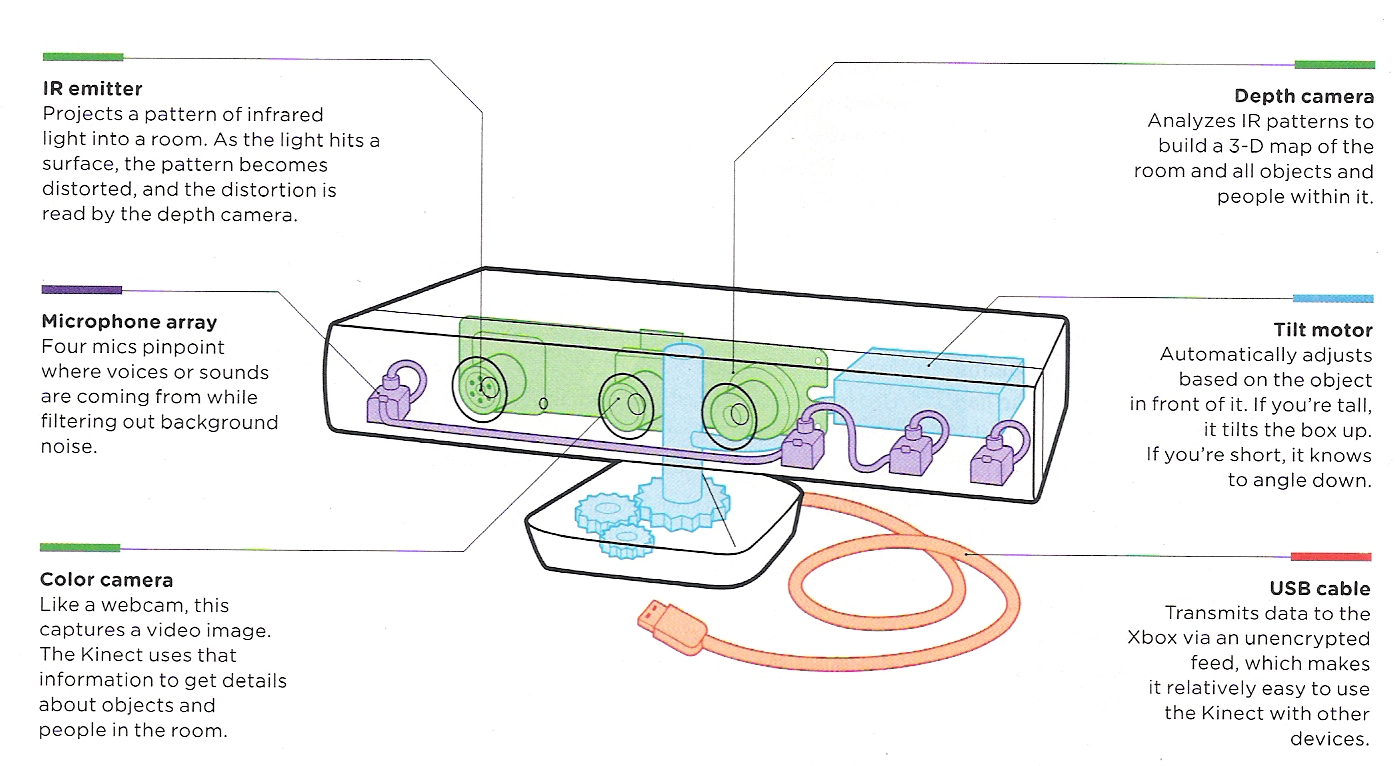
\includegraphics[width=0.80\textwidth]{./figures/Kinect.png}
	\captionof{figure}{Composição do Kinect}
	\label{fig:5}
\end{center}

O \emph{Kinect} tem, como se pode ver na figura~\ref{fig:5}, uma câmara normal RGB 
contudo os sensores que extraem a perceção de profundidade é a câmara de infra-vermelhos à direita
que capta os infra-vermelhos enviados pelo emissor situado à esquerda.

Entretanto foi lançado no \emph{Windows SDK} um controlador e uma \emph{framework} oficiais para se desenvolver aplicações fazendo uso do \emph{Kinect} na plataforma \emph{Windows}.


\section{Técnicas de Reconhecimento de Objetos}\label{objdetect}

Nesta secção do documento apresenta-se e explora-se as técnicas mais
promissoras de deteção e reconhecimento de objetos em imagens 2D e
em estruturas de representação em 3D que assumem a maior importância 
no âmbito do ramo científico da visão por computador.

\subsection[SIFT]{Scale Invariant Feature Transform}\label{sift}

\emph{Scale-Invariant Feature Transform} (SIFT) \cite{Lowe:1999:ORL:850924.851523} é uma técnica para o reconhecimento de objetos bastante popular em computação visual. Para fazer o reconhecimento de objetos, esta técnica necessita de um treino prévio, onde são extraídas características que não variam com a escala, rotações nem com projeções em 3D, sendo também parcialmente resistente a diferenças em iluminação.

A qualidade desta técnica está dependente da qualidade das características que extrai, e do facto de estas serem invariantes apesar das transformações que se possa aplicar à imagem.

A extração de características é feita em vários passos. O primeiro é e
aplicação da função gaussiana na direção horizontal a todas as linhas de pixeis
 e de seguida na vertical em todas as colunas.
É utilizada também uma pirâmide de imagens onde se fez uma progressiva interpolação bilinear para suavizar a imagem, sendo que  a função gaussiana é aplicada a
todas as camadas de modo a que cada uma seja comparada às suas adjacentes
para determinar os máximos e os mínimos.

\[
g(x) = \frac{1}{\sqrt{2\pi\sigma}}e^{-x^3 / 2 \sigma^2}
\]

O resultado desta análise é um conjunto de vetores que representam as
características do objeto. 


\begin{center}
	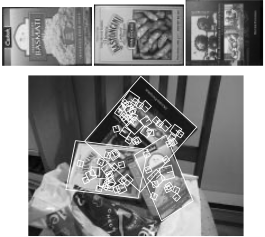
\includegraphics[scale=1.00]{figures/sift_img.png}
	\captionof{figure}{Exemplo de Detecção utilizando SIFT}
	\label{fig:1}
\end{center}

\subsection[SURF]{Speeded Up Robust Feature}

Speeded Up Robust Feature (SURF) é uma técnica bastante próxima de SIFT\ref{sift}, contudo tem a vantagem de ser mais robusta às transformações que se pode fazer às imagens conseguindo também, ao mesmo tempo, aumentar a performance e a repetibilidade da deteção nas imagens \cite{citeulike:973069}.

As melhorias enunciadas são conseguidas através da escolha cuidadosa dos pontos característicos de um objeto. Esta escolha é feita utilizando o conceito de imagens integrais \cite{10.1109CVPR.2001.990517} cujo conceito básico é que cada pixel $x$ na imagem inicial é a soma dos valores dos pixeis no retângulo formado pela origem da imagem e as coordenadas do pixel atual:

\[
I_\sum(x) = \sum_{i \leq x}^{i=0} \sum_{j \leq y}^{j=0} I(i,j)
\]


A vantagem destas imagens integrais é que são necessárias apenas adições
para calcular a soma das intensidades em qualquer área retangular vertical.

Os pontos característicos são encontrados onde o determinante de uma matriz
hessiana é máxima.


\subsection{Geometric Hashing}

O \emph{geometric hashing}, tal como os métodos acima representados é uma técnica baseada
em modelos pré-existentes que visa reconhecer objetos onde são aplicadas rotações,
translações e escala \cite{1989SPIE.1095..515C}

Esta técnica tem por base também pontos característicos que são obtidos por
conjuntos de três pontos não colineares segundo os quais os outros são achados. 
Desta forma os seus pontos característicos não variam de acordo com as 
transformações que possam ser aplicadas aos objetos.

%\subsection{Conditional Random Fields}


\subsection{RANSAC}

RANSAC\cite{Fischler:1981:RSC:358669.358692}, um acrónimo de \emph{RANdom SAmple Consensus}, é um algoritmo que permite extrair, através de um conjunto de dados, os parâmetros do modelo matemático que compõe as características aproximadas do objeto. Este algoritmo funciona de forma iterativa, sendo que a cada iteração melhora a qualidade dos parâmetros extraídos.

Este método representa uma evolução significativa dos métodos mínimos quadrados \footnote{devo referir o método dos mínimos quadrados antes?} visto ser permeável a desvio dos dados sem que estes afetem a qualidade da modelação matemática.
Como se pode ver na figura \ref{fig:ransac_vs_lsq} o método \emph{RANSAC} será um método melhor para uma situação real onde os dados têm muito ruído.


\begin{center}
	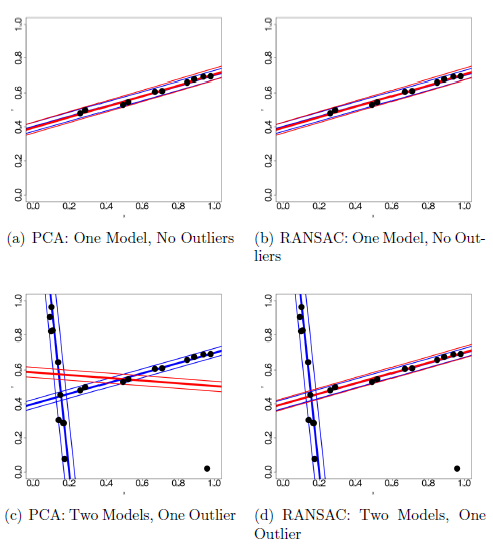
\includegraphics[width=0.80\textwidth]{figures/least_squares_vs_ransac.png}
	\captionof{figure}{Comparação com o método de mínimos quadrados}
	\label{fig:ransac_vs_lsq}
\end{center}



\begin{center}
	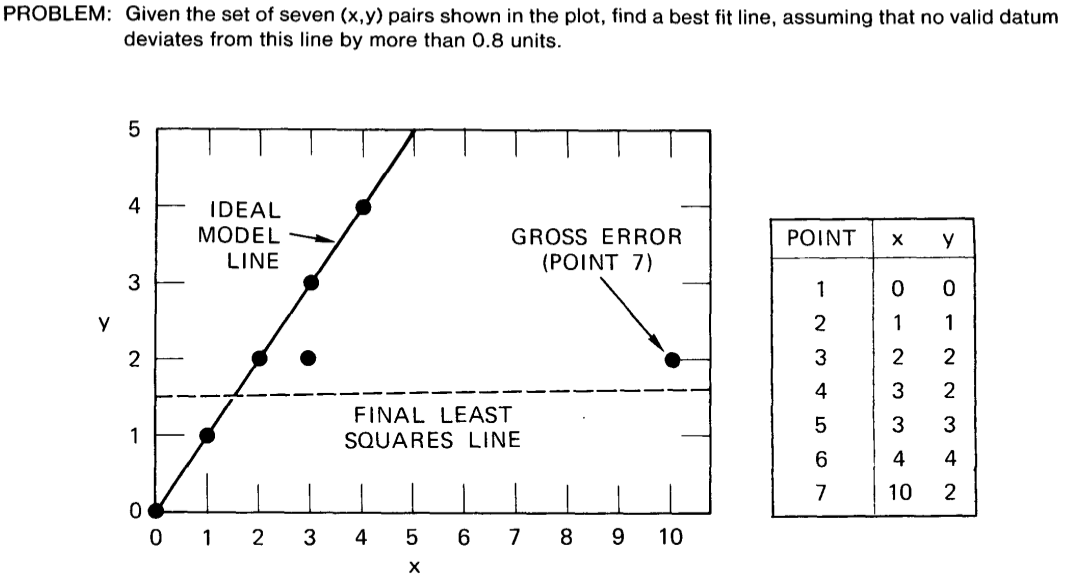
\includegraphics[width=0.80\textwidth]{figures/least_squares_shortcomings.png}
	\captionof{figure}{Exemplo de fraqueza do método de mínimos quadrados}
	\label{fig:ransac}
\end{center}


\subsection[PCL]{Point Cloud Library}

\emph{Point Cloud Library} (PCL) é um projecto \emph{opensource} desenvolvido em C++ cujo objetivo é disponibilizar uma ferramenta altamente otimizada para capturar, manipular, visualizar e processar nuvens de pontos. Nuvens de pontos são a informação 3D que sensores como o \emph{Kinect}\ref{kinect} devolvem, que não é mais do que a nuvem dos pontos captados no espaço, com a origem no ponto onde o sensor se encontra, também com a informação das cores dos pontos.
O projeto PCL \cite{Rusu_ICRA2011_PCL} permite que
através da nuvem de pontos se extraia a informação desejada, sendo que
já tem implementado um conjunto de filtros, técnicas de reconstrução de
superfícies, métodos de extração de características 3D (por exemplo
normais às superfícies), que a tornam uma ferramenta de muito interessante para usar a par do \emph{Kinect}.

A captura de imagens é bastante facilitada com esta ferramenta, que disponibiliza um formato para que toda a informação seja guardada convenientemente: \emph{.pcd}. Estes ficheiros podem ser visualizados facilmente recorrendo a bibliotecas de visualização da PCL onde são apresentados em 3D, sendo que podem conter só informação de profundidade como na figura~\ref{fig:pcl_depth}, mas também com toda a informação capturada pelo \emph{Kinect} como pode ser visto na figura~\ref{fig:pcl_color}.

\begin{center}
	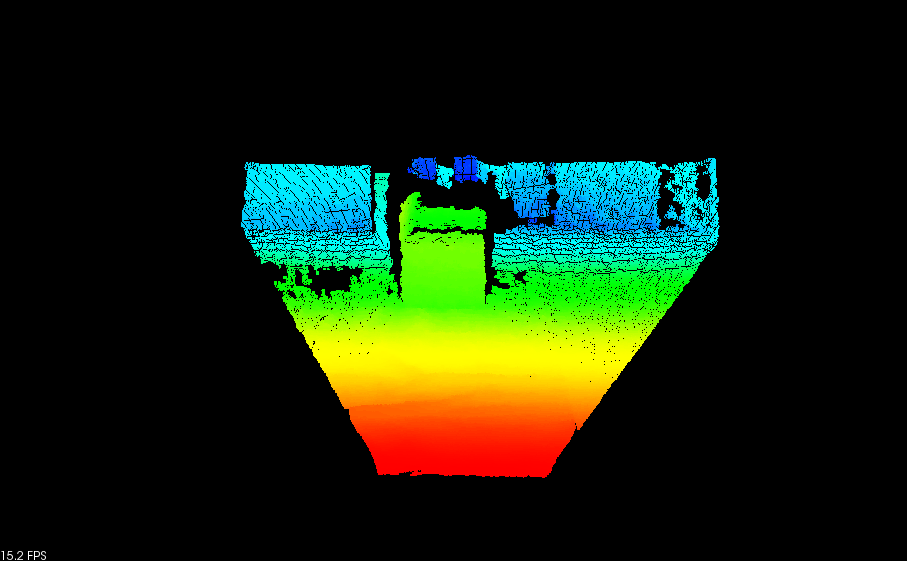
\includegraphics[width=0.80\textwidth]{figures/pcl_openni.png}
	\captionof{figure}{Exemplo de imagem capturada só com a informação de profundidade}
	\label{fig:pcl_depth}
	
\end{center}

\begin{center}
	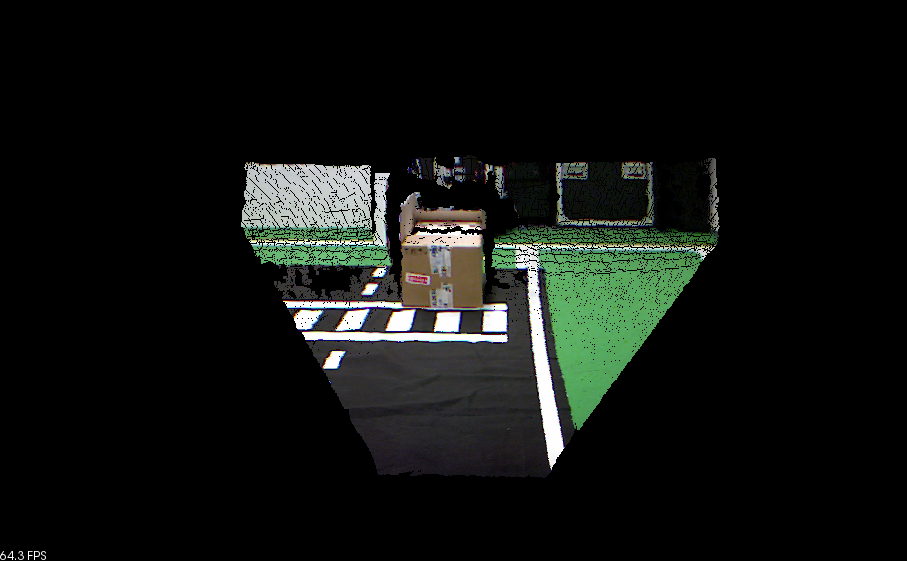
\includegraphics[width=0.80\textwidth]{figures/pcl_color.png}
	\captionof{figure}{Exemplo de imagem capturada com informação RGBD}
	\label{fig:pcl_color}
	
\end{center}


\section{Algoritmos de Clustering}~\ref{sec:clustering}

Tendo-se já explorado algoritmos de identificação de objetos e os sensores, é conveniente também uma abordagem aos algoritmos de \emph{clustering}, isto porque numa dada imagem em 3D, o que existe são uma série de pontos distribuídos no espaço com a informação de cor, sendo então necessário distinguir quais pertencem a um dado objeto e não a outro.

As técnicas de \emph{clustering} permite que se distribua os pontos por uma série de grupos de acordo com uma série de características dos mesmo e de algumas pré-condições fornecidas.

São expostas nesta secção algumas técnicas de \emph{clustering}, nomeadamente as que apresentam mais vantagens e conveniência para esta dissertação.

\subsection{k-d tree}

O algoritmo k-d tree, é um algoritmo de clustering....


\section{Demonstradores de Robótica Autónoma}
Esta secção refere-se a demonstradores de robótica autónoma, onde são referidos
os exemplos que traduzem o que se está a fazer no âmbito de demonstradores de
robótica autónoma e que representam o estado da arte nesta área.


\subsection{DARPA: Grand Challenge}
A agência norte americana DARPA (\emph{Defense Advanced Research Agency}), cujos projetos de
investigação se destinam principalmente a aplicações militares, realizou três grandes
eventos onde foram postos à prova as técnicas de condução autónoma de veículos
comerciais devidamente equipados e modificados para se poderem mover de uma forma
completamente autónoma.  

Existiram duas edições do \emph{Grand Challenge} realizadas em 2004 e 2005 que consistia
numa prova de condução autónoma em que os carros percorriam uma estrada de cerca
de 242km no deserto do \emph{Mojave}. Em 2004 nenhum dos concorrentes chegou ao final da
prova, sendo que o o robô que mais distância percorreu ficou pelos 18km, contudo em 2005

Em 2007 foi realizado um \emph{Urban Challenge} onde se aproximou as provas às condições
encontradas num ambiente urbano, ou seja, estradas com carros a circular em ambas as
vias, cruzamentos, sinalização vertical  e semáforos.

Na edição de 2007 os veículos autónomos estão equipados com um conjunto de sensores
 entre os quais se destacam LIDAR, Radares, sonares e infravermelhos. O projeto
vencedor desenvolvido pela Universidade de \emph{Carnegie Mellon} e apelidado de
 \emph{Boss} \cite{Urmson:2008:ADU:1395073.1395077} tem
18 sensores dispostos como apresentado no diagrama abaixo:

\begin{center}
	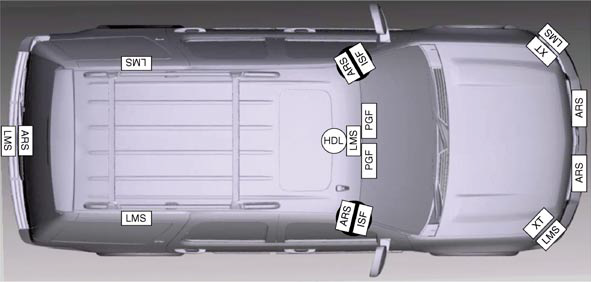
\includegraphics[width=0.80\textwidth]{./figures/boss_sensors.png}
	\captionof{figure}{Sensores no Boss \cite{Urmson:2008:ADU:1395073.1395077}.}
	\label{fig:2}
\end{center}

\begin{table}
\begin{center}
\begin{tabular} { c c l }
	Sigla & Tipo de Equipamento & Modelo \\
	\hline
	APLX & GPS & Applanix POS-LV 220/420 GPS/IMU \\
	LMS & LIDAR & SICK LMS 291-S05/S14 LIDAR \\
	HDL & LIDAR & Velodyne HDL-64 LIDAR \\
	ISF & LIDAR & Continental ISF 172 LIDAR \\
	XT & LIDAR & IBEO Alasca XT LIDAR \\
	ARS & RADAR & Continental ARS 300 Radar \\
	PGF & Câmara HDR & Point Grey Firefly \\
	\hline
\end{tabular}
	\caption{Listagem dos sensores do \emph{Boss}}
	\label{boss_sensor}
\end{center}
\end{table}

Sendo que os códigos dos sensores correspondem ao indicado na tabela ~\ref{boss_sensor}
pode-se concluir, que os sensores LIDAR são um excelente sensor para ajudar no reconhecimento
de objectos no mundo, tal como para mapear o ambiente do robô para se poder orientar de uma eficaz.


\subsection{Festival Nacional de Robótica}

O festival nacional de robótica é um evento organizado anualmente pela sociedade
portuguesa de robótica em cidades diferentes onde, além de um encontro de científico
onde investigadores de robótica de todo o mundo discutem e apresentam os trabalhos
que estão a desenvolver, são realizadas várias competições e demonstrações de robótica.

As competições que se realizam são as seguintes:
\begin{itemize}
\item    Busca e Salvamento Júnior RoboCup
\item    Dança Júnior RoboCup
\item    Futebol Robótico Júnior RoboCup
\item    Condução Autónoma
\item    Liga INFAIMON Futebol Robótico Médio RoboCup
\item    FreeBots
\item    Robot@Factory
\item    Equipas
\item    Qualificações para o RoboCup
\end{itemize}

Destas competições, a mais relevante para o trabalho a ser desenvolvido no 
âmbito desta dissertação é a de Competição Autónoma, onde um robô totalmente 
autónomo tem de navegar numa pista em oito que tem as características apresentadas:

\begin{center}
	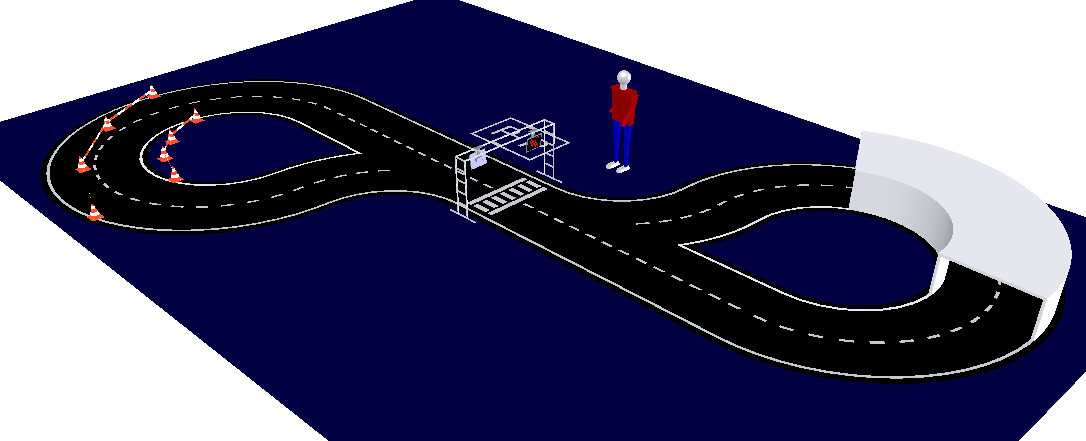
\includegraphics[width=1.00\textwidth]{./figures/ca_pista.png}
	\captionof{figure}{Pista de Condução Autónoma no Festival Nacional de Robótica}
	\label{fig:3}
\end{center}

O objetivo é o robô percorrer a pista circulando pela faixa da direita, seguindo
as indicações no sinais verticais que se situam à beira da pista e os semáforos,
e evitar os obstáculos que sinalizam obras no percurso.


\subsection{MINERVA}
O minerva é um robô autónomo desenvolvido na universidade Carnegie Mellon, para
fazer de robô guia no museu Smithsonian para a exposição de história natural que
esteve em exibição no período de 25 de Agosto a 5 de Setembro de 1998.

\begin{center}
	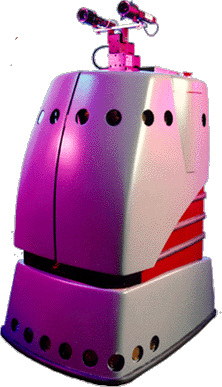
\includegraphics[width=0.20\textwidth]{./figures/minerva.png}
	\captionof{figure}{MINERVA - Robô guia do museu Smithsonian}
	\label{fig:4}
\end{center}

Este robô era totalmente autónomo a partir do momento em que fazia uma volta de
aprendizagem, em que era guiado pelo percurso que lhe estava destinado. Estando
a aprendizagem concluída, o robô orientava-se pelo resultado da sua aprendizagem,
e por alguns sensores, nomeadamente para se desviar dos visitantes e de obstáculos,
uma câmara para detetar marcadores no teto do museu para se conseguir localizar.
Além de guiar os visitantes pelo percurso este robô também interagia com os mesmos,
respondendo a perguntas e apresentando a exposição.

\subsection{CleanRob}

O CleanRob é um projeto que começou a ser desenvolvido na Faculdade de Engenharia da 
Universidade do Porto em 2004, no no contexto do Departamento de Engenharia
Eletrotécnica e de Computadores. Este robô foi desenvolvido por alunos de modo a
envolver alunos no desenvolvimento de projetos académicos com maior aplicação prática
tirando partido de técnicas que representam o estado da arte na robótica.

Este robô utiliza um conjunto de câmaras e sonares PSD para fazer a sua localização,
de modo a limpar corredores do departamento de Engenharia Eletrotécnica.

\begin{center}
	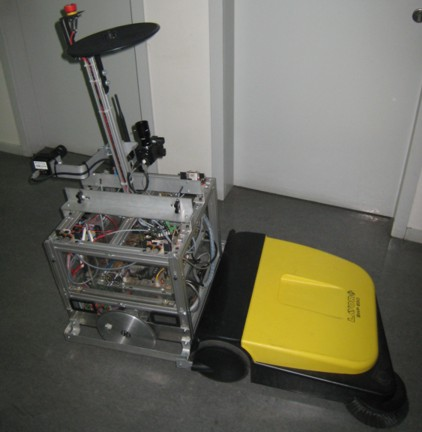
\includegraphics[width=0.40\textwidth]{./figures/clean_rob.jpg}
	\captionof{figure}{CleanRob}
	\label{fig:6}
\end{center}


\section{Resumo}

No que diz respeito a deteção de objetos, existem vários algoritmos bastante robustos e
eficazes, contudo são muito voltados para reconhecimento em imagens RGB
e não tanto baseados em conjuntos de dados 3D e além disso exigem uma fase de aprendizagem.

Os demonstradores autónomos que existem no momento já são bastante completos, considere-se
como exemplo o \emph{Boss} que navega em ambiente bastante próximo do urbano com proeza,
estando cada vez mais próximo de um cenário onde condução autónoma nas cidades poderia ser
uma realidade e até mesmo uma mais-valia em termos de segurança. É de assinalar também os esforços
nas competições de robôs em escalas menores pois com menos recursos e menor escala consegue-se
testar técnicas inovadoras com soluções menos dispendiosas obtendo-se resultados igualmente
impressionantes.


\chapter{Visualização de Sinópticos SVG}\label{chap:chap3}

\section*{}

Este capítulo deve começar por fazer uma apresentação detalhada do
problema a resolver\footnote{Na introdução a apresentação do
  problema foi breve.} podendo mesmo, caso se justifique,
constituir-se um capítulo com essa finalidade.

Deve depois dedicar-se à apresentação da solução sem detalhes de
implementação. 
Dependendo do trabalho, pode ser uma descrição mais teórica, mais
``arquitectural'', etc.

\section{Secção Exemplo}

Neste capítulo apresentam-se exemplos de formatação de figuras e
tabelas, equações e referências cruzadas.

Apresenta-se de seguida um exemplo de equação, completamente fora do contexto:
\begin{eqnarray}
CIF_1: \hspace*{5mm}F_0^j(a) &=& \frac{1}{2\pi \iota} \oint_{\gamma} \frac{F_0^j(z)}{z - a} dz\\
CIF_2: \hspace*{5mm}F_1^j(a) &=& \frac{1}{2\pi \iota} \oint_{\gamma} \frac{F_0^j(x)}{x - a} dx \label{eq:cif}
\end{eqnarray}

Na Equação~\ref{eq:cif} lorem ipsum dolor sit amet, consectetuer
adipiscing elit. Suspendisse tincidunt viverra elit. Donec tempus
vulputate mauris. Donec arcu. Vestibulum condimentum porta
justo. Curabitur ornare tincidunt lacus. Curabitur ac massa vel ante
tincidunt placerat. Cras vehicula semper elit. Curabitur gravida, est
a elementum suscipit, est eros ullamcorper quam, sed cursus velit
velit tempor neque. Duis tempor condimentum ante.

Phasellus imperdiet, orci vel pretium sollicitudin, magna nunc
ullamcorper augue, non venenatis dui nunc quis massa. Pellentesque
dolor elit, dapibus venenatis, viverra ultricies, accumsan cursus,
orci. Aliquam erat volutpat. Mauris ornare tristique leo. Maecenas
eros. Curabitur velit nunc, tincidunt vitae, dictum posuere, pulvinar
nec, diam. In suscipit mauris a nunc. Pellentesque gravida. Morbi quam
lacus, pretium eget, tincidunt vulputate, interdum sed,
turpis. Curabitur quis est. Sed lectus lorem, congue vel, dignissim
laoreet, blandit a, nisi. Aenean nunc ligula, tincidunt eu, hendrerit
vel, suscipit non, erat. Aliquam gravida. Integer non pede. In laoreet
augue id leo. Mauris placerat. 

A arquitectura do visualizador assenta sobre os seguintes conceitos
base~\citep{kn:ZPMD97}: 

\begin{itemize}
\item \textbf{Componentes} --- Suspendisse auctor mattis augue \emph{push};
\item \textbf{Praesent} --- Sit amet sem maecenas eleifend facilisis leo;
\item \textbf{Pellentesque} --- Habitant morbi tristique senectus et netus.
\end{itemize}

\subsection{Exemplo de Figura}

É apresentado na Figura~\ref{fig:arch} %da página~\pageref{fig:arch}
um exemplo de figura flutuante.

\begin{figure}[t]
  \begin{center}
    \leavevmode
    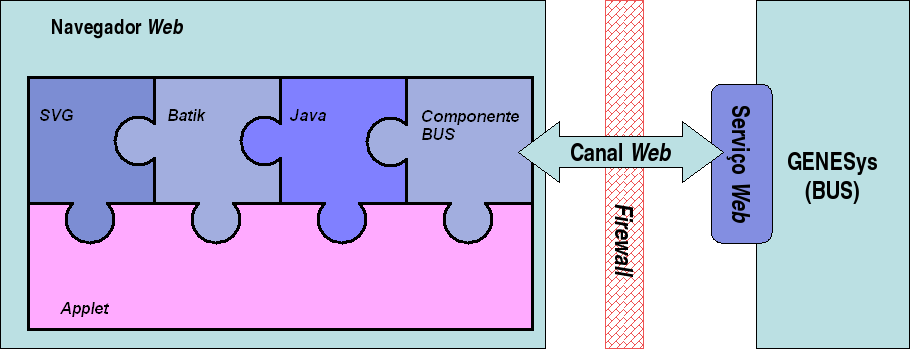
\includegraphics[width=0.86\textwidth]{puzzle}
    \caption{Arquitectura da Solução Proposta}
    \label{fig:arch}
  \end{center}
\end{figure}

Loren ipsum dolor sit amet, consectetuer adipiscing elit. 
Praesent sit amet sem. Maecenas eleifend facilisis leo. Vestibulum et
mi. Aliquam posuere, ante non tristique consectetuer, dui elit
scelerisque augue, eu vehicula nibh nisi ac est. Suspendisse elementum
sodales felis. Nullam laoreet fermentum urna. 

Duis eget diam. In est justo, tristique in, lacinia vel, feugiat eget,
quam. Pellentesque habitant morbi tristique senectus et netus et
malesuada fames ac turpis egestas. Fusce feugiat, elit ac placerat
fermentum, augue nisl ultricies eros, id fringilla enim sapien eu
felis. Vestibulum ante ipsum primis in faucibus orci luctus et
ultrices posuere cubilia Curae; Sed dolor mi, porttitor quis,
condimentum sed luctus. 

\subsection{Exemplo de Tabela}

É apresentado na Tabela~\ref{tab:exemplo1} um exemplo de tabela
flutuante e na Tabela~\ref{tab:exemplo2} um exemplo de tabela
flutuante, um pouco mais complicada.

\begin{table}[t]
  \centering
  \caption{Uma Tabela Simples}
\begin{tabular}{| l | p{45mm} |}
	\hline
\textbf{Acrónimo} & \textbf{Significado}\\
	\hline
	\hline
        ADT   & \emph{Abstract Data Type}\\\hline
        ANDF  & \emph{Architecture-Neutral Distribution Format}\\\hline
        API   & \emph{Application Programming Interface}\\
	\hline
\end{tabular}
  \label{tab:exemplo1}
\end{table}

Integer quis pede. Fusce nibh. Fusce nec erat vel mi condimentum
convallis. Sed at tortor non mauris pretium aliquet. In in lacus in
dolor molestie dapibus. Suspendisse potenti. Pellentesque sagittis
porta erat. Mauris sodales sapien id augue. Nam eu dolor. Donec sit
amet turpis non orci rhoncus commodo. Etiam condimentum commodo
libero.

Mauris pede. Curabitur faucibus dictum nibh. Proin tincidunt diam
vitae mauris. Sed hendrerit dolor vel ipsum. Nullam dapibus. Vivamus
tellus diam, egestas sit amet, vulputate non, vulputate id, eros. Nunc
sit amet nibh eget nibh imperdiet ornare. Cras vehicula mattis
ipsum. Sed diam arcu, semper at, gravida vitae, fermentum et,
nulla. Aenean massa orci, tristique nec, rutrum id, fringilla eget,
erat. Curabitur nulla ipsum, aliquam sed, rutrum vitae, semper quis,
ante. Fusce at nunc in dolor condimentum tempor. Duis sit amet massa. 

Curabitur convallis nulla quis risus. Nulla mollis porttitor
purus. Fusce ultricies odio at ligula pellentesque suscipit. Nulla
velit libero, blandit a, aliquet quis, hendrerit id, arcu. Phasellus
porttitor porttitor purus. Suspendisse velit tortor, fringilla sit
amet, commodo a, ultrices et, mi. Donec eu metus in erat ornare
adipiscing. Praesent varius mi ac nunc. Vestibulum leo lacus,
elementum in, vestibulum sit amet, hendrerit at, justo. Sed sit amet
neque. Donec libero risus, commodo sit amet, dignissim ut, tincidunt
a, eros. Ut non lacus quis tortor mattis ullamcorper. Vivamus
consequat augue vel erat. Sed tincidunt. Sed leo eros, ornare a,
pulvinar non, mattis quis, nibh. Aliquam faucibus mi ac nisi.

Pellentesque habitant morbi tristique senectus et netus et malesuada
fames ac turpis egestas. Duis aliquet, libero sit amet ornare viverra,
augue erat interdum dolor, vitae tincidunt lorem erat a lacus. Sed
lectus nisi, auctor in, hendrerit a, molestie vel, lectus. Cum sociis
natoque penatibus et magnis dis parturient montes, nascetur ridiculus
mus. Duis lacinia tempor dui. Vivamus rhoncus, tellus a viverra
dignissim, pede dui adipiscing odio, non faucibus metus mi gravida
eros. Nullam a tellus ut velit elementum tempus. Aenean rutrum
convallis tellus. Vestibulum nulla ante, dapibus ut, lobortis ut,
varius sed, nisl. Fusce lobortis. Sed ac lorem. Nulla tincidunt nulla
eget leo. Maecenas ac lectus eu neque ultrices pharetra. Curabitur a
risus nec arcu placerat tempor. Suspendisse magna nisl, viverra a,
adipiscing eget, ornare ultricies, ligula. Maecenas eu ligula vitae
eros convallis dignissim. 

\begin{table}[t]
  \centering
  \caption{Uma Tabela Mais Complicada}
\begin{tabular}{|c|r@{.}lr@{.}lr@{.}l||r|}
	\hline
\multicolumn{8}{|c|}
	{\rule[-3mm]{0mm}{8mm}Iteração $k$ de $f(x_n)$} \\
\textbf{\em k}
	& \multicolumn{2}{c}{$x_1^k$}
	& \multicolumn{2}{c}{$x_2^k$}
	& \multicolumn{2}{c||}{$x_3^k$}
	& comentários \\ \hline \hline
0   & -0&3                 & 0&6                 &  0&7   & - \\
1   &  0&47102965 & 0&04883157 & -0&53345964  & $\delta<\epsilon$ \\
2   &  0&49988691 & 0&00228830 & -0&52246185  & $\delta < \varepsilon$ \\
3   &  0&49999976 & 0&00005380 & -0&523656   &   $N$ \\
4   &  0&5                 & 0&00000307 & -0&52359743  & \\
\vdots	& \multicolumn{2}{c}{\vdots}
	& \multicolumn{2}{c}{$\ddots$}
	& \multicolumn{2}{c||}{\vdots}  & \\
7   &  0&5   & 0&0    & \textbf{-0}&\textbf{52359878}
		 & $\delta<10^{-8}$ \\ \hline
\end{tabular}
  \label{tab:exemplo2}
\end{table}

Loren ipsum dolor sit amet, consectetuer adipiscing elit. 
Praesent sit amet sem. Maecenas eleifend facilisis leo. Vestibulum et
mi. Aliquam posuere, ante non tristique consectetuer, dui elit
scelerisque augue, eu vehicula nibh nisi ac est. Suspendisse elementum
sodales felis. Nullam laoreet fermentum urna. 

Duis eget diam. In est justo, tristique in, lacinia vel, feugiat eget,
quam. Pellentesque habitant morbi tristique senectus et netus et
malesuada fames ac turpis egestas. Fusce feugiat, elit ac placerat
fermentum, augue nisl ultricies eros, id fringilla enim sapien eu
felis. Vestibulum ante ipsum primis in faucibus orci luctus et
ultrices posuere cubilia Curae; Sed dolor mi, porttitor quis,
condimentum sed luctus. 

\section{Secção Exemplo}

Loren ipsum dolor sit amet, consectetuer adipiscing elit. 
Praesent sit amet sem. Maecenas eleifend facilisis leo. Vestibulum et
mi. Aliquam posuere, ante non tristique consectetuer, dui elit
scelerisque augue, eu vehicula nibh nisi ac est. Suspendisse elementum
sodales felis. Nullam laoreet fermentum urna. 

Duis eget diam. In est justo, tristique in, lacinia vel, feugiat eget,
quam. Pellentesque habitant morbi tristique senectus et netus et
malesuada fames ac turpis egestas. Fusce feugiat, elit ac placerat
fermentum, augue nisl ultricies eros, id fringilla enim sapien eu
felis. Vestibulum ante ipsum primis in faucibus orci luctus et
ultrices posuere cubilia Curae; Sed dolor mi, porttitor quis,
condimentum sed luctus. 

\section{Resumo e Conclusões}

Resumir e apresentar as conclusões que se podem tirar no fim deste
capítulo.

\chapter{Implementação}\label{chap:chap4}

% \section*{}
% Este capítulo pode ser dedicado à apresentação de detalhes de nível
% mais baixo relacionados com o enquadramento e implementação das
% soluções preconizadas no capítulo anterior.
% Note-se no entanto que detalhes desnecessários à compreensão do
% trabalho devem ser remetidos para anexos.

% Dependendo do volume, a avaliação do trabalho pode ser incluída neste
% capítulo ou pode constituir um capítulo separado.

A ideia principal do projeto seria fazer a deteção de objetos simples e depois capitalizar nessa capacidade desenvolvida para fazer a deteção de objetos mais complexos. Esta deteção de objetos, que culminou na escolha da mesa como caso de estudo, pelas considerações que já foram explanadas da sua morfologia, tem como objetivo último a sua utilização num demonstrador de robótica autónoma, fazendo recurso a um dicionário pré-existente em que as mesas conhecidas são listadas num ficheiro \emph{XML}.

O programa desenvolvido foi escrito em \emph{C++} recorrendo a algumas bibliotecas informáticas, nomeadamente a \emph{Point Cloud Library} (PCL) para a captura e manipulação de nuvens de pontos e a \emph{Boost} porque além de ser um requisito da PCL tem uma miríade de bibliotecas auxiliares implementadas que potenciam o desenvolvimento e trazem uma garantia de terem a melhor performance possível. De seguida são analisados com mais detalhe os pormenores de implementação.

\section{Captura de Imagens 3D para análise }

A captura de imagens em 3D foi desenvolvida utilizando a biblioteca \emph{Point Cloud Library}, e é uma das capacidades do projeto associado a esta dissertação. As nuvens de pontos são guardadas em ficheiros PCD e guardam o que é capturado pelo \emph{Kinect}, sendo que contém toda a informação RGBD e pode ser visualizada com a mesma aplicação que as gerou.

\begin{center}
	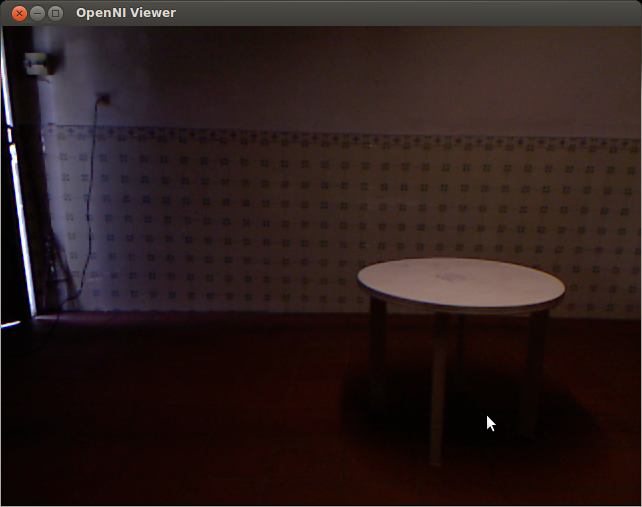
\includegraphics[width=0.8\textwidth]{figures/experiencia/exp4.png}\\
	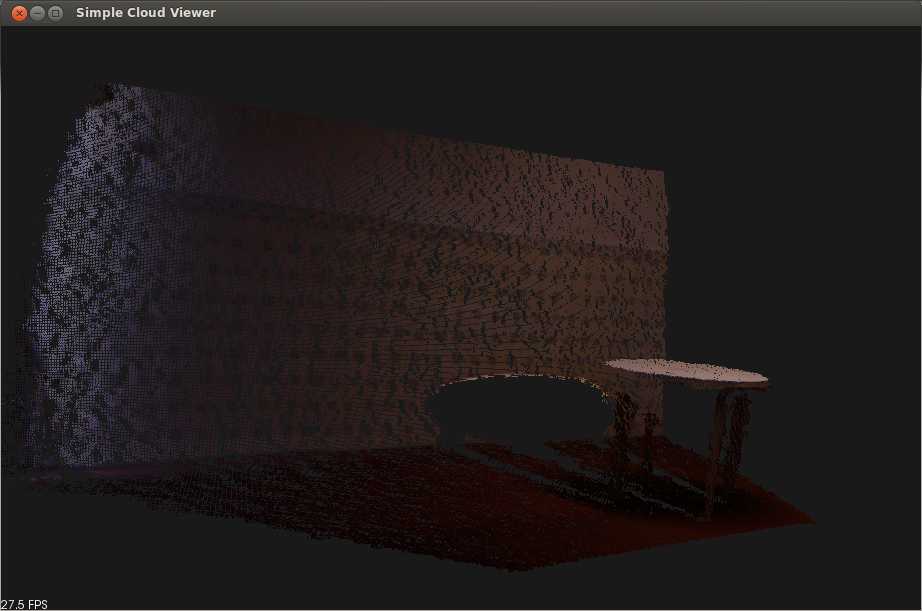
\includegraphics[width=0.4\textwidth]{figures/exemplo_captura_perspectiva1.png}
	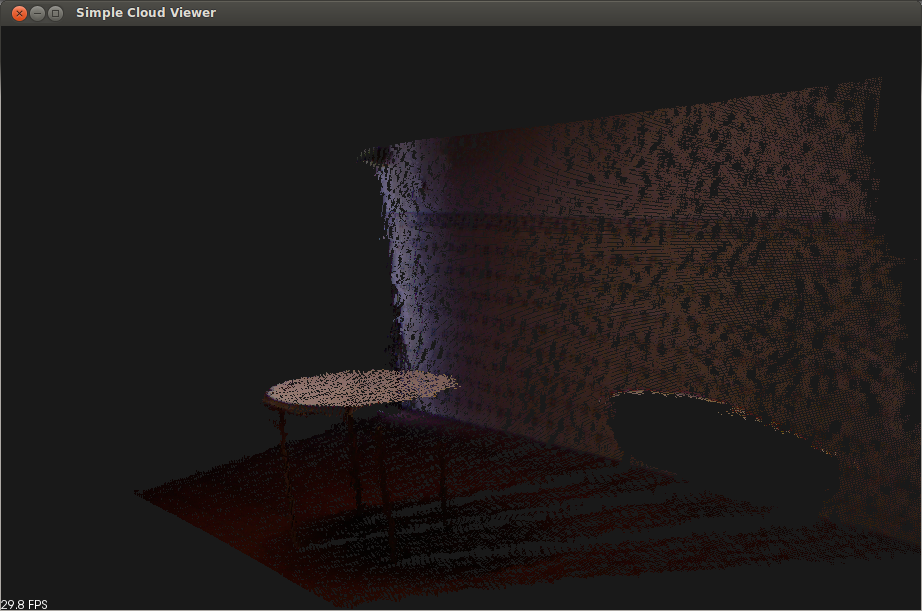
\includegraphics[width=0.4\textwidth]{figures/exemplo_captura_perspectiva2.png}

	\captionof{figure}{Exemplo de imagem capturada com informação RGBD (duas perspetivas) e a imagem RGB correspondente.}
	\label{fig:exemplo_captura}
\end{center}


\section{Estudo de Precisão do Kinect}

Antes de se passar à implementação da deteção, considerou-se necessário fazer um estudo da precisão das medições do Kinect de modo a garantir que as análises das imagens, e qualquer consideração prévia, estariam corretas e não se baseavam em suposições.

Sendo assim escolheu-se um objeto e mudou-se a sua posição relativa ao \emph{Kinect}. Em cada uma das posições registadas, foram medidas e guardadas as distâncias e os ângulos, sendo que de seguida foram registadas doze imagens RGBD por posição e submeteu-se cada uma a uma análise automatizada para medir a distância e o ângulo ao objeto.

A sequencia dos registos encontra-se na tabela~\ref{res:dist_analise} que se encontra abaixo.

\begin{table}[htb]
	\begin{center}
		\begin{tabular} { l c c c}
			Nº da Posição & Distância ( m ) & Ângulo ( $^\circ$ ) \\
			\hline
			1 & 1.35 & 0 \\
			2 &  1.34 & 21\\
			3 & 2.00 & 0 \\
			4 & 1.93 & 14 \\
			5 & 2.30 & -27\\
			6 & 2.75 & 0 \\
			7 & 2.75 & 18 \\
			8 & 3.00 & -18 \\
			\hline
		\end{tabular}
		\caption{Experiências à precisão do Kinect}
		\label{res:dist_analise}
	\end{center}
\end{table}

A posição da mesa relativamente ao \emph{Kinect} para cada posição pode ser verificado na figura~\ref{fig:exp_posicoesmesa}.

\begin{center}
	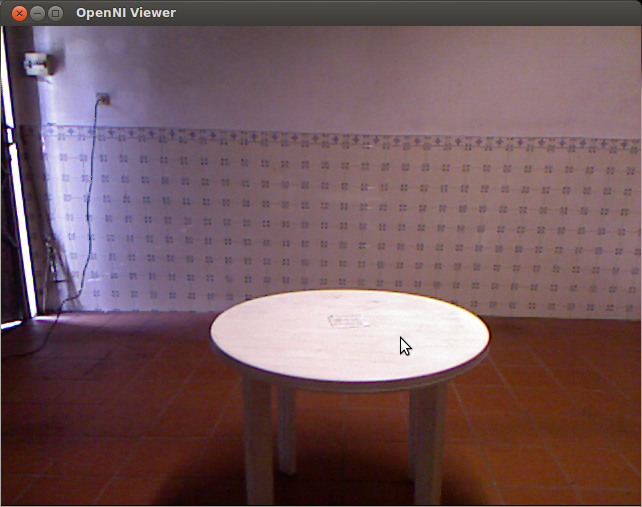
\includegraphics[width=0.240\textwidth]{figures/experiencia/exp1.png}
	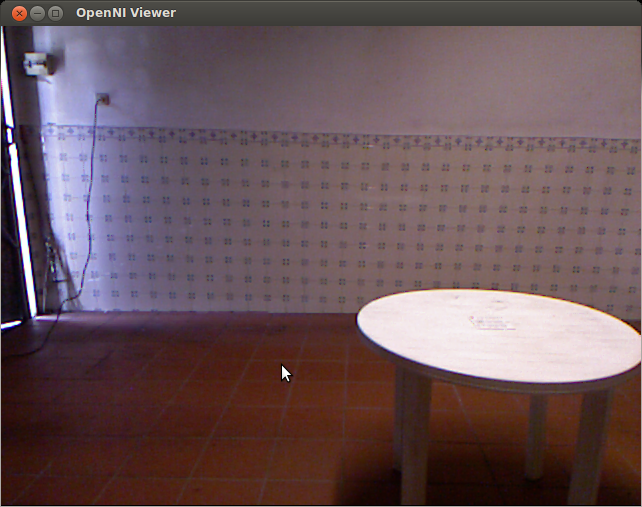
\includegraphics[width=0.240\textwidth]{figures/experiencia/exp2.png}
	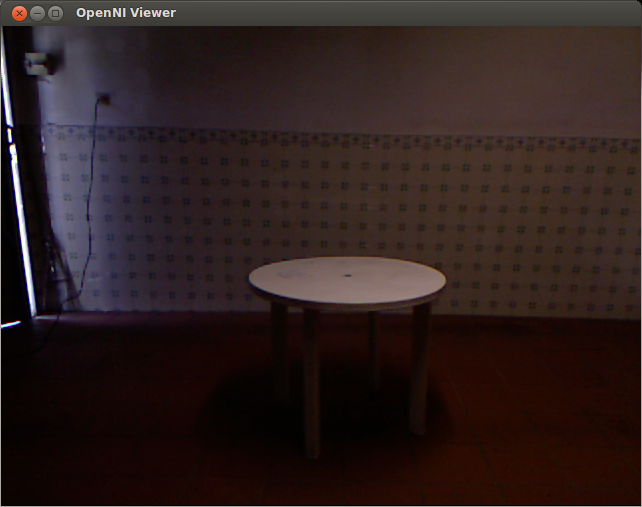
\includegraphics[width=0.240\textwidth]{figures/experiencia/exp3.png}
	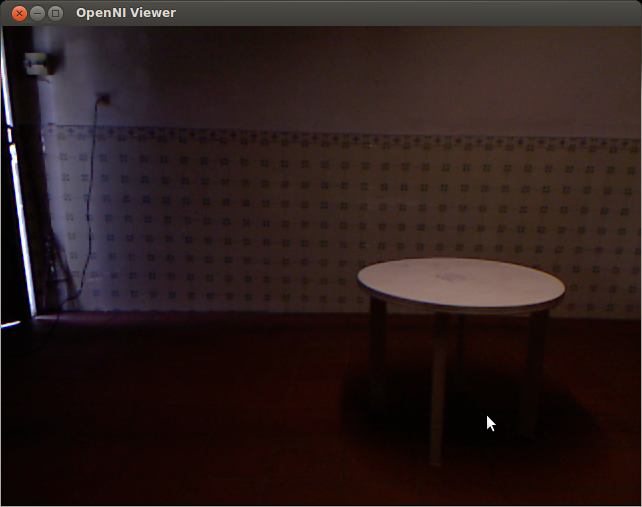
\includegraphics[width=0.240\textwidth]{figures/experiencia/exp4.png} \\
	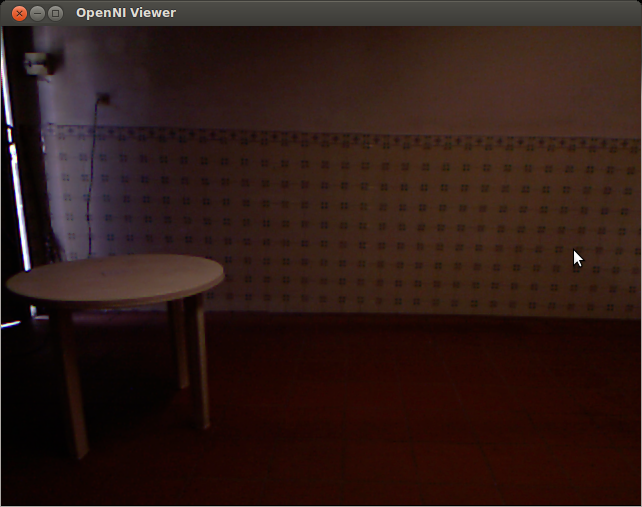
\includegraphics[width=0.240\textwidth]{figures/experiencia/exp5.png}
	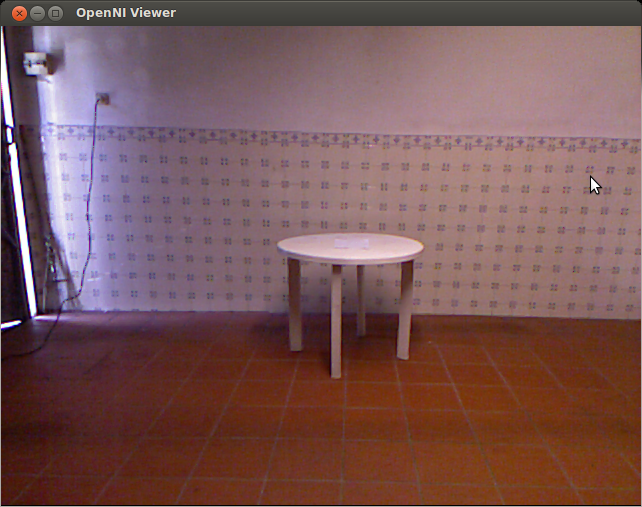
\includegraphics[width=0.240\textwidth]{figures/experiencia/exp6.png}
	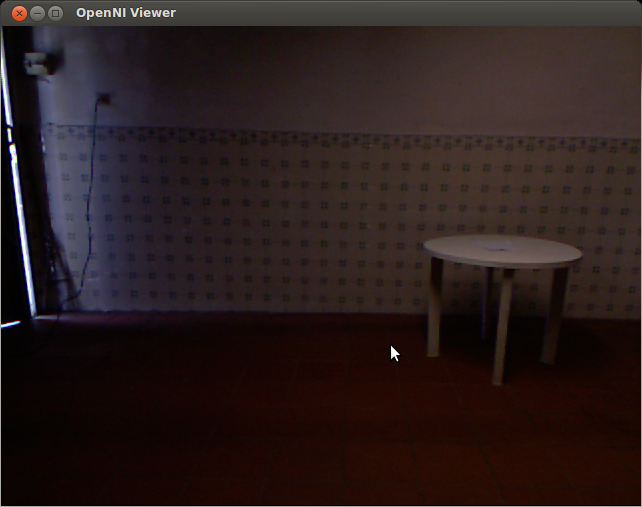
\includegraphics[width=0.240\textwidth]{figures/experiencia/exp7.png}
	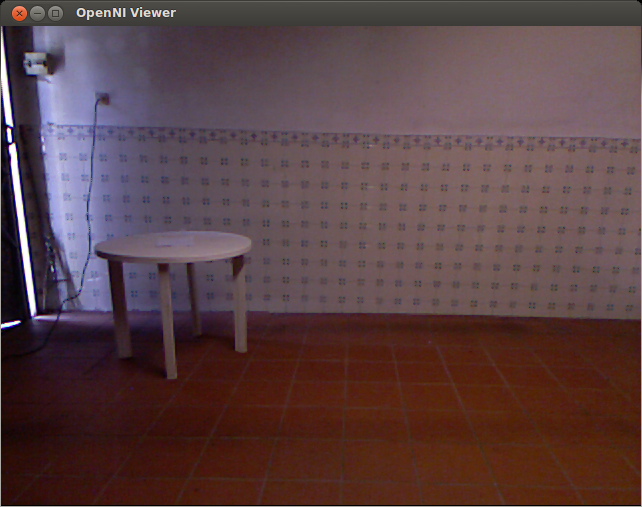
\includegraphics[width=0.240\textwidth]{figures/experiencia/exp8.png}
	\captionof{figure}{Foto das posições da mesa relativas ao Kinect.}
	\label{fig:exp_posicoesmesa}
\end{center}


De seguida para cada imagem de cada posição avaliou-se qual a distância do \emph{Kinect} à mesa que a imagem RGBD regista. Os resultados encontram-se registados na tabela~\ref{res:exp_res_obtidos} sendo que para cada uma das posições criou-se um diagrama temporal para avaliar quanto as posições registada pelo \emph{Kinect} se desviam da posição medida fisicamente, que se encontram apresentados nas figuras ~\ref{fig:chart_1} a ~\ref{fig:chart_8}.


\begin{table}[!htb]
\begin{center}
\begin{tabular} { c c c c c c c c }

\hline
\multicolumn{8}{c}{ Posições ( m ) }\\
\hline
 1 & 2 & 3 & 4 & 5 & 6 & 7 & 8 \\
\hline
1.35 & 1.339247 & 1.975414 & 1.910938 & 2.413945 & 2.762543 & 2.753629 & 3.023028 \\
1.35754 & 1.334866 & 1.952989 & 1.931228 & 2.377091 & 2.76339 & 2.750247 & 3.060131 \\
1.362351 & 1.334632 & 1.985518 & 1.931326 & 2.38616 & 2.786931 & 2.771791 & 3.059977 \\
1.35799 & 1.339735 & 1.985523 & 1.931682 & 2.36845 & 2.786493 & 2.791635 & 3.062525 \\
1.358089 & 1.339071 & 1.975026 & 1.931579 & 2.380317 & 2.791077 & 2.771245 & 3.059977 \\
1.35759 & 1.339247 & 1.974677 & 1.930731 & 2.380086 & 2.78675 & 2.770061 & 3.042213 \\
1.357634 & 1.334736 & 1.985874 & 1.942546 & 2.380075 & 2.786312 & 2.791803 & 3.044104 \\
1.358572 & 1.338895 & 1.987369 & 1.931143 & 2.344773 & 2.812669 & 2.813004 & 3.04185 \\
1.358485 & 1.334144 & 1.987345 & 1.931502 & 2.351119 & 2.786493 & 2.791803 & 3.04185 \\
1.355191 & 1.339556 & 1.974662 & 1.931858 & 2.376915 & 2.700064 & 2.771245 & 3.02285 \\
1.358148 & 1.339383 & 1.98587 & 1.942116 & 2.353092 & 2.790619 & 2.817074 & 3.02285 \\
1.357711 & 1.339069 & 1.98587 & 1.942461 & 2.348412 & 2.720287 & 2.794201 & 3.022684 \\
\hline
\end{tabular}
	\caption{Resultados obtidos das distâncias para cada posição}
	\label{res:exp_res_obtidos}
\end{center}
\end{table}


\begin{figure}
\begin{center}
	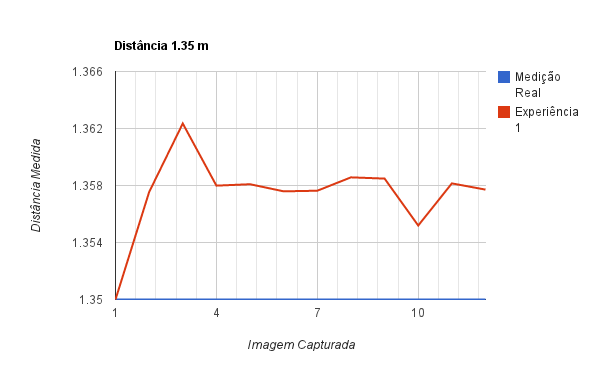
\includegraphics[width=0.80\textwidth]{figures/experiencia/chart_1.png}
	\captionof{figure}{Diagrama temporal para a primeira posição (1.35 m)}
	\label{fig:chart_1}
\end{center}
\end{figure}

\begin{figure}
\begin{center}
	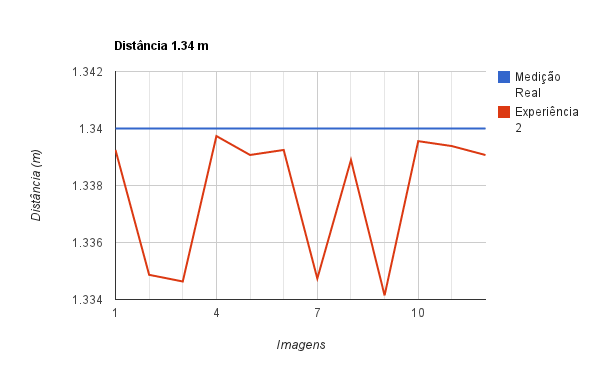
\includegraphics[width=0.80\textwidth]{figures/experiencia/chart_2.png}
	\captionof{figure}{Diagrama temporal para a segunda posição (1.34 m)}
	\label{fig:chart_2}
\end{center}
\end{figure}

\begin{figure}
\begin{center}
	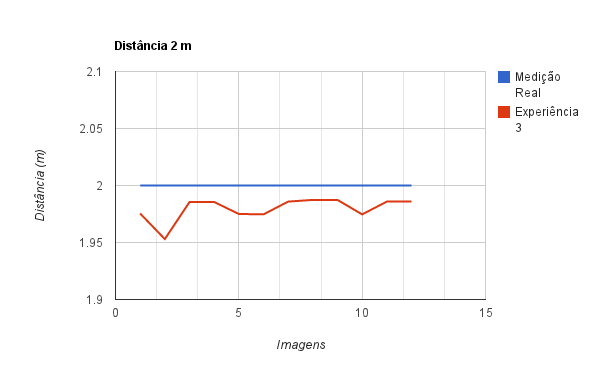
\includegraphics[width=0.80\textwidth]{figures/experiencia/chart_3.png}
	\captionof{figure}{Diagrama temporal para a terceira posição (2.00 m)}
	\label{fig:chart_3}
\end{center}
\end{figure}

\begin{figure}
\begin{center}
	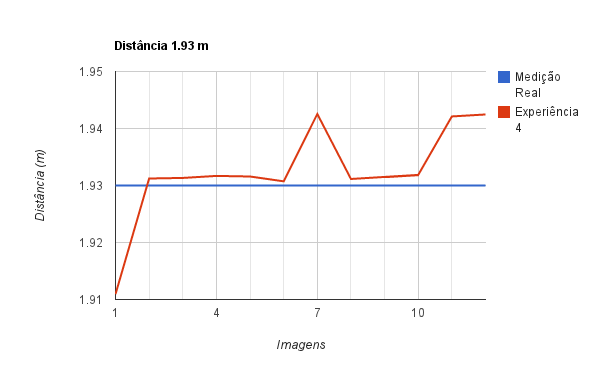
\includegraphics[width=0.80\textwidth]{figures/experiencia/chart_4.png}
	\captionof{figure}{Diagrama temporal para a quarta posição (1.93 m)}
	\label{fig:chart_4}
\end{center}
\end{figure}

\begin{figure}
\begin{center}
	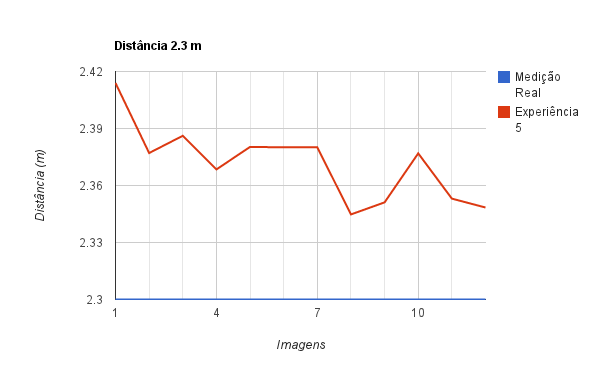
\includegraphics[width=0.80\textwidth]{figures/experiencia/chart_5.png}
	\captionof{figure}{Diagrama temporal para a quinta posição (2.30 m)}
	\label{fig:chart_5}
\end{center}
\end{figure}

\begin{figure}
\begin{center}
	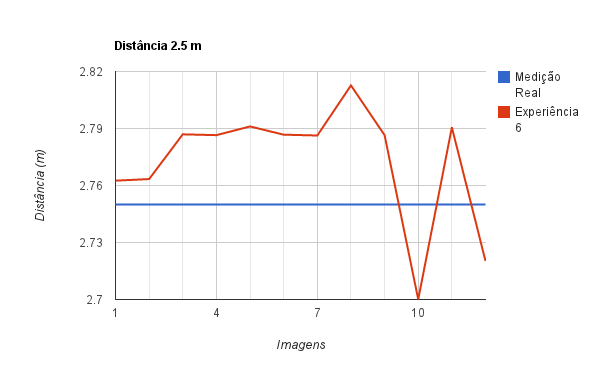
\includegraphics[width=0.80\textwidth]{figures/experiencia/chart_6.png}
	\captionof{figure}{Diagrama temporal para a sexta posição (2.75 m)}
	\label{fig:chart_6}
\end{center}
\end{figure}

\begin{figure}
\begin{center}
	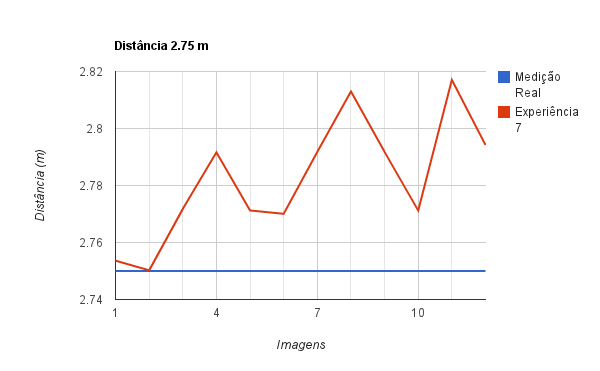
\includegraphics[width=0.80\textwidth]{figures/experiencia/chart_7.png}
	\captionof{figure}{Diagrama temporal para a sétima posição (2.75 m)}
	\label{fig:chart_7}
\end{center}
\end{figure}

\begin{figure}
\begin{center}
	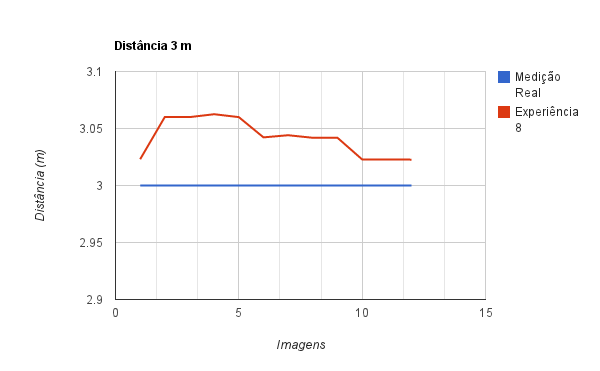
\includegraphics[width=0.80\textwidth]{figures/experiencia/chart_8.png}
	\captionof{figure}{Diagrama temporal para a oitava posição (3.00 m)}
	\label{fig:chart_8}
\end{center}
\end{figure}

Para aprofundar a análise, extraiu-se alguns dados estatísticos das medições que se encontram na tabela~\ref{res:exp_res_obtidos_est} 


\begin{table}[!h]
\begin{center}
\begin{tabular} { c c c c }
Posição & Média ( m ) & Desvio Padrão ( m ) & Mediana ( m ) \\
\hline
1 & 1.3574 & 0.0017 & 1.3579 \\
2 & 1.3377 & 0.0024 & 1.3391\\
3 & 1.9797 & 0.0104 & 1.9855 \\
4 & 1.9324 & 0.0051 & 1.9315 \\
5 & 2.3717 & 0.0154 & 2.3770 \\
6 & 2.7728 & 0.0336 & 2.7865 \\
7 & 2.7823 & 0.0200 & 2.7817 \\
8 & 3.0420 & 0.0157 & 3.0420 \\
\hline
\end{tabular}
	\caption{Dados estatísticos da recolha de distâncias.}
	\label{res:exp_res_obtidos_est}
\end{center}
\end{table}

Olhando para o desvio padrão, percebe-se que a variação dos dados do \emph{Kinect} para a posição do objeto não é muito grande, sendo no máximo de 2 centímetros, contudo houve uma variação algo significativa para o valor medido mas não era demasiado grande, sendo que se considerou bastante aceitável.


Quanto aos ângulos, fez-se uma análise semelhante à das distâncias, cujos resultados são os apresentados nas tabelas \ref{res:exp_res_obtidos_ang} e \ref{res:exp_res_obtidos_est_ang}.

\begin{table}[!h]
\begin{center}
\begin{tabular} { c c c c c c c c }

\hline
 \multicolumn{8}{c}{ Ângulos ( $^\circ$ ) }\\
\hline
1 & 2 & 3 & 4 & 5 & 6 & 7 & 8 \\
\hline
 -15.357386 & 4.792201 &-9.630516 & 4.790509 & -34.3685 & -4.143964 & 14.146553 & -25.240545 \\
 -15.223657 & 4.976701 & -9.608464 & 4.506991 & -34.520763 & -4.379865 & 13.799928 & -24.792519 \\
 -15.168276 & 4.835194 & -9.448602 & 4.506991 & -34.371037 & -4.460659 & 13.811712 & -24.792519 \\
 -15.301353 & 4.932463 & -9.449469 & 4.63898 & -34.216621 & -4.343729 & 13.708774 & -24.889385\\
 -15.301353 & 4.700834 & -9.563814 & 4.63898 & -34.165874 & -5.161427 & 13.811712 & -24.792519\\
 -15.223657 & 4.792201 & -9.501884 & 4.317291 & -34.626232 & -4.460659 & 13.69715 & -25.071798\\
 -15.238359 & 4.994671 & -9.510148 & 4.612736 & -34.626232 & -4.343729 & 13.708774 & -25.169027\\
 -15.383727 & 4.584675 & -9.765748 & 4.476339 & -37.209705 & -5.005285 & 13.602537 & -25.071798\\
 -15.370365 & 4.740714 & -9.761795 & 4.607438 & -34.071758 & -4.343729 & 13.708774 & -25.071798\\
 -15.642712 & 4.926197 & -9.501012 & 4.738488 & -34.981014 & -4.604316 & 13.811712 & -25.240545\\
15.318219 & 4.861241 & -9.511069 & 4.451008 & -34.617245 & -5.044734 & 13.94077 & -25.240545\\
-15.250415 & 4.563166 & -9.511069 & 4.581371 & -33.973186 & -4.329277 & 13.935993 & -25.240545\\

\hline
\end{tabular}
	\caption{Resultados obtidos dos ângulos para cada posição}
	\label{res:exp_res_obtidos_ang}
\end{center}
\end{table}



\begin{table}[!h]
\begin{center}
\begin{tabular} { c c c c }
 Posição & Média ( $^\circ$ ) & Desvio Padrão  ( $^\circ$ ) & Mediana  ( $^\circ$ ) \\
\hline
	1 & -15.3150 &0.1279 & -15.3014 \\
	2 & 4.8084 &0.1491 & 4.8137 \\
	3 &  -9.5636 &0.1114 &-9.5111\\
	4 &  4.5723 &0.1152 & 4.5944 \\
	5 & -34.6457 &0.8926 &-34.4459 \\
	6 & -4.5518 & 0.3215 &-4.4203 \\
	7 & 13.8070 & 0.1034 &  13.8058 \\
	8 & -25.0511 & 0.1861 &  -25.0718 \\
\hline
\end{tabular}
	\caption{Dados estatísticos da recolha de ângulos.}
	\label{res:exp_res_obtidos_est_ang}
\end{center}
\end{table}


\begin{table}[!h]
\begin{center}
\begin{tabular} { c c c c }
 Posição & Valor Real ( $^\circ$ ) & Mediana ( $^\circ$ ) & |Valor Real - Mediana| ( $^\circ$ ) \\
\hline
	1 & 0 & -15.3014 & 15.3014 \\
	2 & 21 & 4.8137 & 16.1863 \\
	3 & 0 & -9.5111& 9.5111\\
	4 & 14 & 4.5944 & 9.4056\\
	5 & -27 & -34.4459 & 7.4459 \\
	6 & 0 & -4.4203 & 4.4203 \\
	7 & 18 & 13.8058 & 4.1942 \\
	8 & -18 & -25.0718 & 7.0718 \\
\hline
\end{tabular}
	\caption{Comparação do valor da mediana com o valor real dos ângulos.}
	\label{res:exp_res_obtidos_est_ang_comp}
\end{center}
\end{table}



Comparando o valor da mediana dos valores obtidos pelo \emph{Kinect} aos que foram fisicamente medidos (ver tabela~\ref{res:exp_res_obtidos_est_ang_comp}), consegue-se concluir que a diferença absoluta entre ambos é no máximo 15 graus, o que aliado aos baixo valores do desvio padrão (< 1 grau) é um indicador que o dispositivo é bastante preciso. 

Olhando para os resultados, é possível também afirmar que a medição física dos ângulos provavelmente não estaria completamente alinhada com o foco do \emph{Kinect}.


Além disso utilizou-se a informação extraída dos ângulos para comparar, recorrendo a gráficos, a posição real dos objetos com a posição onde o sensor regista o objeto.

\begin{figure}
\begin{center}
	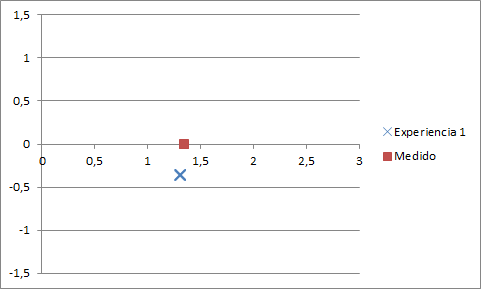
\includegraphics[width=0.80\textwidth]{figures/experiencia/pos_chart_exp1.png}
	\captionof{figure}{Posição real e posições registadas pelo Kinect para a posição 1 (1.35 m)}
	\label{fig:pos_chart_exp1}
\end{center}
\end{figure}

\begin{figure}
\begin{center}
	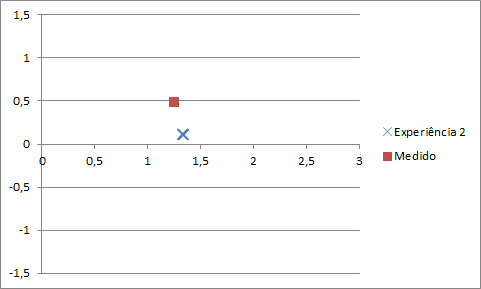
\includegraphics[width=0.80\textwidth]{figures/experiencia/pos_chart_exp2.png}
	\captionof{figure}{Posição real e posições registadas pelo Kinect para a posição 2 (1.34 m)}
	\label{fig:pos_chart_exp2}
\end{center}
\end{figure}

\begin{figure}
\begin{center}
	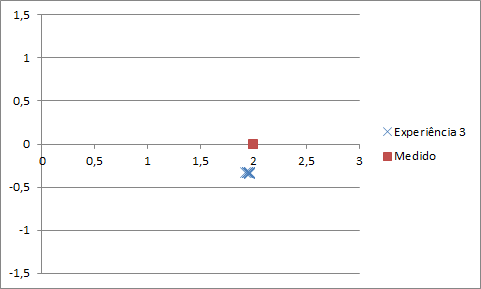
\includegraphics[width=0.80\textwidth]{figures/experiencia/pos_chart_exp3.png}
	\captionof{figure}{Posição real e posições registadas pelo Kinect para a posição 3 (2.00 m)}
	\label{fig:pos_chart_exp3}
\end{center}
\end{figure}

\begin{figure}
\begin{center}
	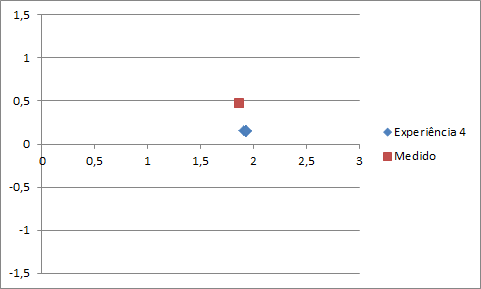
\includegraphics[width=0.80\textwidth]{figures/experiencia/pos_chart_exp4.png}
	\captionof{figure}{Posição real e posições registadas pelo Kinect para a posição 4 (1.93 m)}
	\label{fig:pos_chart_exp4}
\end{center}
\end{figure}

\begin{figure}
\begin{center}
	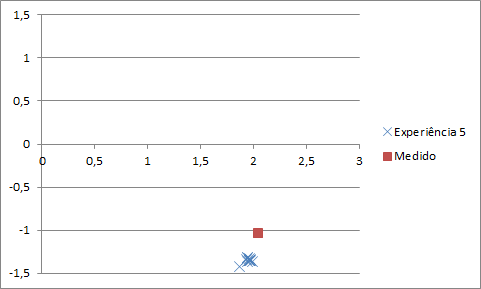
\includegraphics[width=0.80\textwidth]{figures/experiencia/pos_chart_exp5.png}
	\captionof{figure}{Posição real e posições registadas pelo Kinect para a posição 5 (2.30 m)}
	\label{fig:pos_chart_exp5}
\end{center}
\end{figure}

\begin{figure}
\begin{center}
	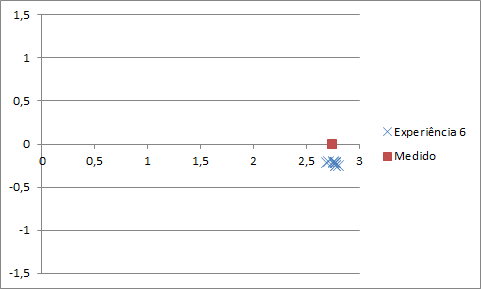
\includegraphics[width=0.80\textwidth]{figures/experiencia/pos_chart_exp6.png}
	\captionof{figure}{Posição real e posições registadas pelo Kinect para a posição 6 (2.75 m)}
	\label{fig:pos_chart_exp6}
\end{center}
\end{figure}

\begin{figure}
\begin{center}
	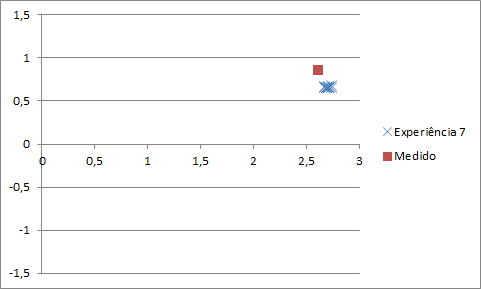
\includegraphics[width=0.80\textwidth]{figures/experiencia/pos_chart_exp7.png}
	\captionof{figure}{Posição real e posições registadas pelo Kinect para a posição 7 (2.75 m)}
	\label{fig:pos_chart_exp7}
\end{center}
\end{figure}

\begin{figure}
\begin{center}
	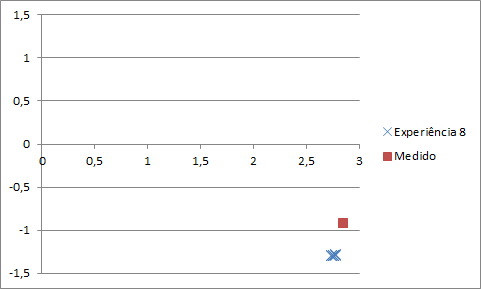
\includegraphics[width=0.80\textwidth]{figures/experiencia/pos_chart_exp8.png}
	\captionof{figure}{Posição real e posições registadas pelo Kinect para a posição 8 (3.00 m)}
	\label{fig:pos_chart_exp8}
\end{center}
\end{figure}


\vspace*{12mm}


\section {Implementação da Deteção}

Agora serão listados todos os passos por que passa uma imagem RGBD para se poder detetar a existência de mesas na nuvem de pontos.

Antes de tudo a informação RGB é descartada pois não tem uma grande influência sobre deteção, isto porque após considerações cuidadosas chegou-se à conclusão que a cor não é um aspeto que tenha grande peso na caracterização da mesa.

Adicionalmente o dicionário de mesas conhecidas é lido a partir do ficheiro \emph{dictionary.xml} e guardado em memória para se poder fazer a comparação com o que é encontrado na imagem e dar um valor que avalia a confiança com que pode garantir que é a mesa indicada.

O ficheiro de dicionário, onde se podem descrever as mesas do dicionário, tem a seguinte gramática:

\begin{description}
	\item [table] - Este é o nó principal que contém os nós com as descrições da mesa;
	\item [name] - Onde é guardado o nome representativo da mesa;
	\item [top] - Onde estão contidos os atributos do tampo que tem a seguinte estrutura:
	\begin{description} 
		\item [shape] - Palavra descritiva da forma do tampo da mesa;
		\item [large\_dimension] - A maior distância medida no tampo em metros; 
		\item [small\_dimension] - A menor distância medida no tampo em metros;
	\end{description} 
	\item [legs] - Onde estão contidos os atributos das pernas da mesa que tem os seguintes parâmetros:
	\begin{description} 
		\item [number] - O número de pernas que a mesa tem;
		\item [height] -  A altura das pernas em metros;
		\item [parallel] - Se as pernas são paralelas ou não;
		\item [center\_distance] - distância das pernas ao centro da mesa.
	\end{description} 
\end{description}

Em suma, as características das mesas são distribuídas entre o tampo da mesa e as pernas, descrevendo a sua morfologia em tanto parâmetros quantitativos como a altura e dimensões dos tampos como em parâmetros qualitativos como a geometria do tampo e se as pernas são paralelas.


\subsection{Pré Processamento}

Agora que se trabalha sobre a informação de profundidade, que se encontra em SI (metros), é feito um pré processamento onde se descarta tudo que aparece na imagem que dista a mais de 4,5 metros do sensor. Isto é no sentido de eliminar erros persistentes na imagem, pois o \emph{Kinect} vai perdendo precisão com a distância \cite{s120201437}. No passo seguinte vai-se remover o maior plano que corresponde ao chão, de modo a isolar os objetos que se encontrem na imagem.


Depois é feita uma clusterização usando o algoritmo de vizinhança Euclidiana para separar o que resta da imagem em objetos coerentes e separáveis. Isto, dando um exemplo prático, é para não acontecer o caso de estarmos a reconhecer o que parece uma perna de uma mesa a dois metros de distância do que é reconhecido como um tampo.

No final deste pré processamento o resultado será um conjunto de nuvens de pontos, em que cada uma representa um objeto que se encontra na imagem capturada inicial.

\begin{figure}[htb]
\begin{center}
	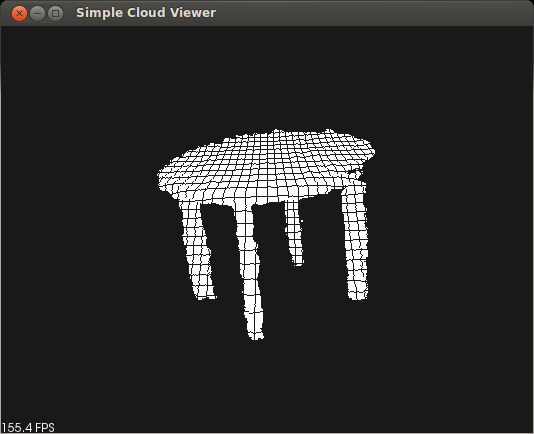
\includegraphics[width=0.80\textwidth]{figures/mesa1_1.png}
	\captionof{figure}{Exemplo de imagem após pré processamento.}
	\label{fig:exemplo_processado}
\end{center}
\end{figure}

\subsection{Deteção de Mesas}

De seguida cada um dos objetos separados passa por um processo onde se tenta detetar constituintes das mesas, como pernas e tampos. Caso sejam encontrados verifica-se se correspondem a alguma das mesas conhecidas que estão guardadas no dicionário das mesas conhecidas, retornando um valor de de confiança \(C\) que se encontra sempre entre 0 e 1.

Esta deteção é feita nos seguintes passos: primeiro faz-se a deteção do tampo, que é obrigatoriamente uma superfície planar, e caso não tenha um plano é logo atribuída uma confiança de 0, considerando-se que não é uma mesa, pois considera-se que caso exista um plano então existirá um tampo. A deteção do plano é feito recorrendo a um conjunto de métodos da PCL que devolvem o conjunto de pontos que pertencem ao plano e as suas características matemáticas.  

 Para avaliar a confiança (\(C_t\)) de o tampo da mesa ser o do modelo que está no dicionário, é seguida a seguinte formulação para cada uma das características (\(C_i\)):

\begin{equation}\label{eq:ci}
C_i = 1 - \frac{|valor\_modelo - valor\_observado|}{valor\_modelo}
\end{equation}

Chegou-se a esta formulação por se considerar, através da experimentação, que seria a que melhor consideraria todas as características para uma melhor qualidade na identificação.

Sendo que se avalia tanto a dimensão maior \(C_1\) como a mais pequena  \(C_2\) e são ambas igualmente relevantes para a avaliação do ajuste da mesa observada vão ter ambas um peso de 0.5 na avaliação do tampo, portanto o valor da confiança \(C_t\) é calculado através da seguinte fórmula:

\begin{equation}\label{eq:ct}
C_t = 0.5C_1 + 0.5C_2
\end{equation}

As dimensões do plano encontrado são avaliadas e comparadas com cada um dos modelos, sendo que a metodologia utilizada para a sua obtenção foi utilizar métodos da PCL para extrair os pontos máximos e mínimos do \emph{cluster} por ele formado e depois utilizá-los para calcular as ditas dimensões.

De seguida é feita uma análise aos apoios. Estes apoios são obtidos através da remoção dos pontos que fazem parte do tampo, restando apenas os pontos que lhes pertencem, sendo de seguida separados utilizando um algoritmo de \emph{clustering}. A confiança dos apoios é representada por \(C_a\) sendo que tem em consideração o número de apoios observados, e a altura dos mesmos. Cada um destes fatores, respetivamente \(C_n\) e \(C_h\), são calculados seguindo a formulação~\ref{eq:ci}. Os valores obtidos são pesados onde a \(C_n\) é aplicado um fator de 0.4 pois facilmente um dos apoios é oculto nas imagens em 3D portanto tem de ter um peso menor, enquanto que a altura \(C_h\) dos apoios tem um peso de 0.6 na avaliação de os apoios corresponderem aos do modelo no dicionário. Em termos de fórmula:

\begin{equation}\label{eq:ca}
C_a = 0.4C_n + 0.6C_h
\end{equation}

Com base no que foi detetado o valor de confiança global é calculado, distribuindo a confiança igualmente pelo que foi calculado quanto ao tampo \(C_t\) e e quanto aos apoios \(C_a\) sendo que a formulação final fica:

\begin{equation}\label{eq:cfinal}
C = 0.5C_t + 0.5C_a
\end{equation}

De seguida analisa-se os resultados que são produzidos pela metodologia descrita, contudo todo este processo encontra-se esquematizado na figura ~\ref{fig:processamento}.

\begin{figure}[!htb]
	\begin{center}
	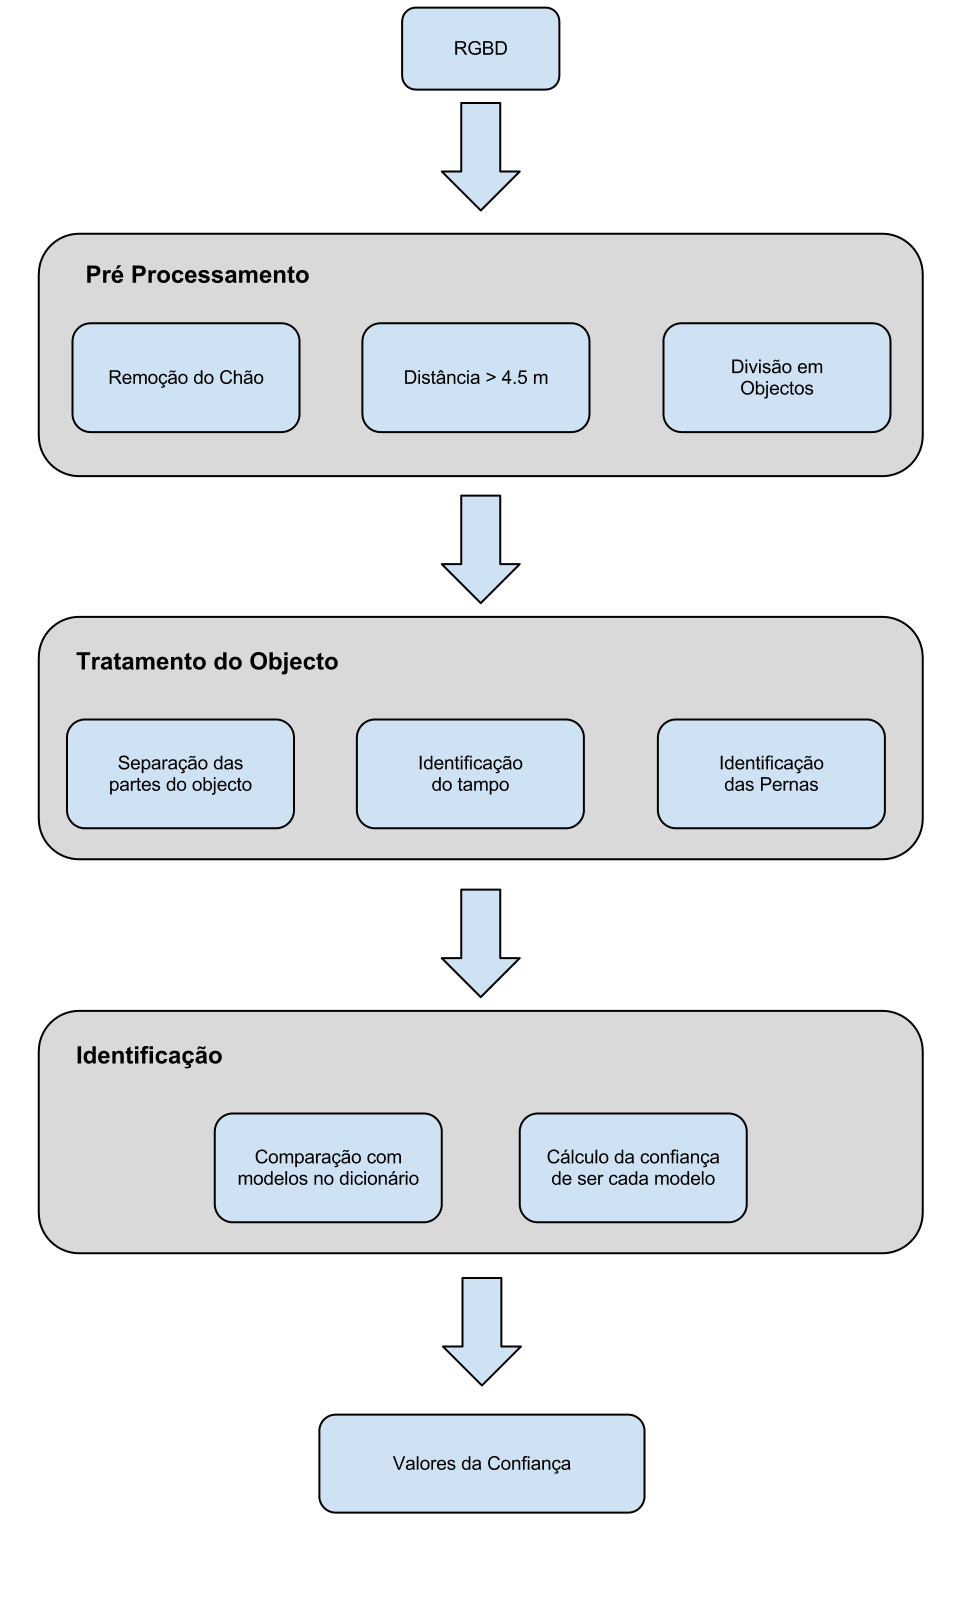
\includegraphics[width=0.80\textwidth]{figures/processo_identificacao.png}
		\captionof{figure}{Funcionamento do processo global.}
		\label{fig:processamento}
	\end{center}
\end{figure}

\vspace*{12mm}




\section {Resultados Obtidos}

Para se obter resultados foram analisadas três mesas diferentes que são descritas no seguinte ficheiro de dicionário em XML. 

\begin{verbatim}
dictionary.xml

<?xml version="1.0" ?>
<table>
	<name>Mesa 1</name>
	<top shape="round" large_dimension="0.89" small_dimension="0.89"/>
	<legs  number="4" height="0.68" parallel="true"/>
</table>
<table>
	<name>Mesa 2</name>
	<top shape="squared" large_dimension="1.0" small_dimension="1.0"/>
	<legs  number="4" height="0.7" parallel="true"/>
</table>
<table>
	<name>Mesa 3</name>
	<top shape="squared" large_dimension="1.0" small_dimension="1.0"/>
	<legs  number="4" height="0.59" parallel="true"/>
</table>
<table>
	<name>Mesa 4</name>
	<top shape="squared" large_dimension="2.0" small_dimension="1.5"/>
	<legs  number="3" height="0.9" parallel="true"/>
</table>
<table>
	<name>Mesa 5</name>
	<top shape="round" large_dimension="1.5" small_dimension="1.5"/>
	<legs  number="1" height="0.8" parallel="true" />
</table>
\end{verbatim}



A primeira mesa, apresentada na figura~\ref{fig:mesa1}, como aparece representado no dicionário, é uma mesa redonda, com aproximadamente 90 centímetros de diâmetro e tem quatro apoios com cerca de 70 centímetros de altura.

\begin{figure}[htb]
\begin{center}
	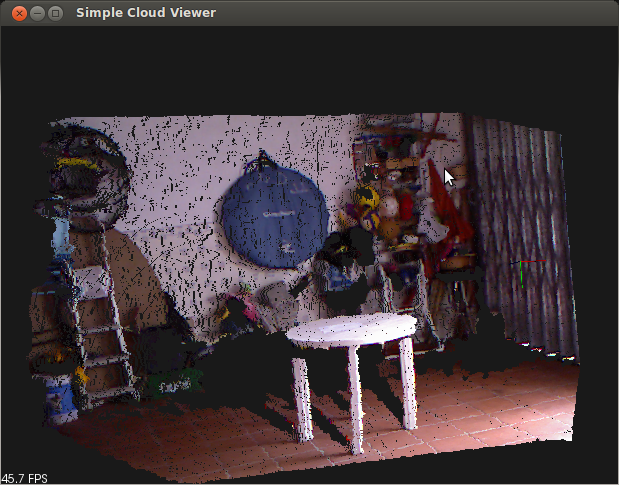
\includegraphics[width=0.80\textwidth]{figures/exemplo_captura.png}
	\captionof{figure}{Primeira mesa a ser identificada.}
	\label{fig:mesa1}
\end{center}
\end{figure}

A segunda mesa a ser identificada é idêntica à primeira mas tem um tampo quadrado de 1 metro de lado, como pode ser observado na figura ~\ref{fig:mesa2}.

\begin{figure}[htb]
\begin{center}
	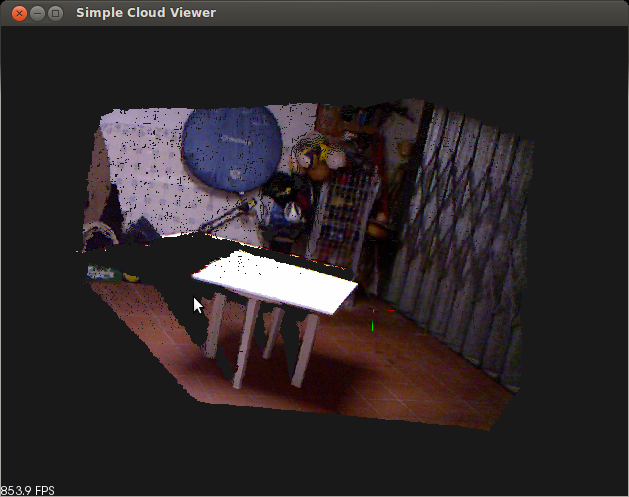
\includegraphics[width=0.80\textwidth]{figures/mesa2.png}
	\captionof{figure}{Segunda mesa a ser identificada.}
	\label{fig:mesa2}
\end{center}
\end{figure}

A terceira mesa (figura ~\ref{fig:mesa3}) é mais baixa com cerca de 60 centímetros de altura e tem quatro apoios. O tampo é quadrado e tem 1 metro de lado.

\begin{figure}[htb]
\begin{center}
	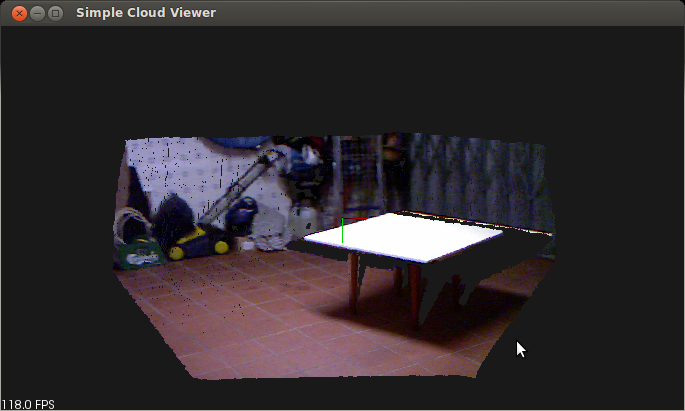
\includegraphics[width=0.80\textwidth]{figures/mesa3.png}
	\captionof{figure}{Terceira mesa a ser identificada.}
	\label{fig:mesa3}
\end{center}
\end{figure}

As mesas 4 e 5 não correspondem a mesas testadas, contudo servem para analisar como é que esta metodologia de reconhecimentos avalia morfologias diferentes.


\begin{table}[htb]
\begin{center}
\begin{tabular} { l | c c c }
	\multicolumn{4}{ c }{ Comparação das mesas}\\
	\hline
	Característica & Mesa 1 & Mesa 2 & Mesa 3 \\
	\hline
	Forma & Circular & Quadrada & Quadrada \\
	Dimensão Maior do Tampo  & 0.89 & 1.0 & 1.0 \\
	Dimensão Menor do Tampo & 0.89 & 1.0 & 1.0 \\
	Numero de Pernas & 4 & 4 & 4 \\
	Altura & 0.68 & 0.7 & 0.59 \\
	Pernas Paralelas & sim & sim & sim \\
	\hline
\end{tabular}
	\caption{Comparação das dimensões das mesas analisadas.}
	\label{res:mesas_comp}
\end{center}
\end{table}

De seguida captou-se uma série de imagens RGBD em várias perspetivas dessas mesas para tentar fazer o reconhecimento.

Os resultados da identificação para cada uma das mesas descritas são apresentados abaixo, sendo que antes se apresenta a significância de cada uma das variáveis:

\begin{itemize}
	\item \(C_1\) - Confiança da dimensão maior;
	\item \(C_2\) - Confiança da dimensão menor;
	\item \(C_n\) - Confiança do número de pernas;
	\item \(C_h\) - Confiança da altura das pernas;
	\item \(C\) - Confiança de ter identificado a mesa analisada;
\end{itemize}


De seguida seguem-se os resultados das experiências feitas, sendo que de uma série de imagens RGBD das três mesas diferentes foram escolhidas três e verificou-se se era possível identificar a mesa correta através da metodologia proposta. É também de notar que as experiências foram realizadas num computador com um processador \emph{Core i7-2630QM} e 8GB  de memória.

\subsection{Identificação}

\begin{table}[htb]
%\caption{Mesa 1}
\begin{center}
\begin{tabular} { c c c c c | c }
	\hline
	Modelo do dicionário & \(C_1\) & \(C_2\) & \(C_n\) & \(C_h\) & \(C\) \\
	\hline
	\multicolumn{6}{ c }{Primeiro Ensaio}\\
	\hline
	Mesa 1 &	 0.997753 &	0.987125 & 1.000000 & 0.702837 & 0.907070 \\
	Mesa 2 &	 0.892000 &	0.878541 & 1.000000 & 0.682756 & 0.847462 \\
	Mesa 3 &	 0.892000 &	0.878541 & 1.000000 & 0.810049 & 0.885650 \\
	Mesa 4 &	 0.446000 &	0.585694 & 0.666667 & 0.531032 & 0.550567 \\
	Mesa 5 &	 0.594667 &	0.585694 & -2.000000 & 0.597411 & 0.074314 \\
	\hline
	\multicolumn{6}{ c }{Segundo Ensaio}\\
	\hline
	Mesa 1 &	 0.938588 &	0.816854 & 0.750000 & 0.785464 & 0.824500 \\
	Mesa 2 &	 0.835343 &	0.727000 & 0.750000 & 0.763022 & 0.769492 \\
	Mesa 3 &	 0.835343 &	0.727000 & 0.750000 & 0.905281 & 0.812170 \\
	Mesa 4 &	 0.417671 &	0.484667 & 1.000000 & 0.593462 & 0.603623 \\
	Mesa 5 &	 0.556895 &	0.484667 & -1.000000 & 0.667645 & 0.260684 \\
	\hline
	\multicolumn{6}{ c }{Terceiro Ensaio}\\
	\hline
	Mesa 1 &	 0.986337 &	0.946067 & 1.000000 & 0.607531 & 0.865360 \\
	Mesa 2 &	 0.902160 &	0.842000 & 1.000000 & 0.590173 & 0.813092 \\
	Mesa 3 &	 0.902160 &	0.842000 & 1.000000 & 0.700205 & 0.846102 \\
	Mesa 4 &	 0.451080 &	0.561333 & 0.666667 & 0.459023 & 0.524144 \\
	Mesa 5 &	 0.601440 &	0.561333 & -2.000000 & 0.516401 & 0.045614 \\
	\hline
\end{tabular}
	\caption{Resultados das análises da Mesa 1}
	\label{res:mesa1}
\end{center}
\end{table}

A análise de uma imagem RGBD da Mesa 1 apresenta resultados bastante satisfatórios, onde o modelo do dicionário com um valor de confiança mais alto é o que na realidade a representa nas três experiências. Verificou-se também que existe pouca diferença entre o valor de confiança do modelo da Mesa 1 e o da Mesa 2, contudo poderá ser explicável pelo facto de as duas mesas com morfologias muito aproximadas.


Adicionalmente os \emph{clusters} representativas das mesas encontram-se na figura~\ref{fig:mesa1_ensaios}.

\begin{figure}[htb]
\begin{center}
	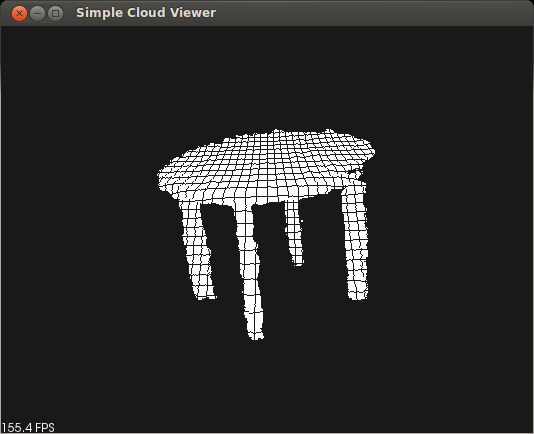
\includegraphics[width=0.30\textwidth]{figures/mesa1_1.png}
	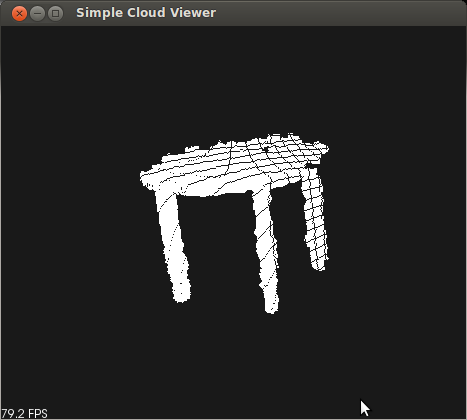
\includegraphics[width=0.30\textwidth]{figures/mesa1_2.png}
	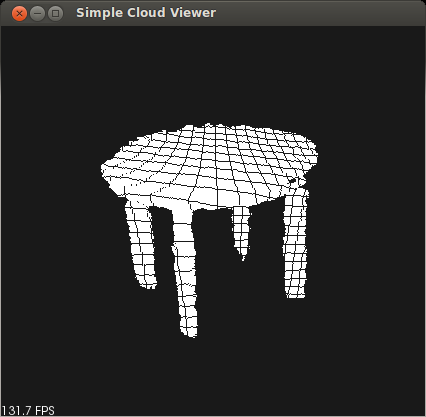
\includegraphics[width=0.30\textwidth]{figures/mesa1_3.png}
	\captionof{figure}{Clusters representativos da mesa 1.}
	\label{fig:mesa1_ensaios}
\end{center}
\end{figure}

\begin{table}[htb]
\begin{center}
\begin{tabular} { c c c c c | c }
	Modelo do dicionário & \(C_1\) & \(C_2\) & \(C_n\) & \(C_h\) & \(C\) \\
		\hline
	\multicolumn{6}{ c }{Primeiro Ensaio}\\
	\hline
	Mesa 1 &	 0.622630 &	0.789887 & 1.000000 & 0.647027 & 0.747238 \\
	Mesa 2 &	 0.774141 &	0.923000 & 1.000000 & 0.628541 & 0.812847 \\
	Mesa 3 &	 0.774141 &	0.923000 & 1.000000 & 0.745726 & 0.848003 \\
	Mesa 4 &	 0.612930 &	0.718000 & 0.666667 & 0.488865 & 0.612725 \\
	Mesa 5 &	 0.817239 &	0.718000 & -2.000000 & 0.549973 & 0.148802 \\
	\hline
	\multicolumn{6}{ c }{Segundo Ensaio}\\
	\hline
	Mesa 1 &	 0.434151 &	0.717978 & 1.000000 & 0.789819 & 0.724978 \\
	Mesa 2 &	 0.606394 &	0.859000 & 1.000000 & 0.767252 & 0.796524 \\
	Mesa 3 &	 0.606394 &	0.859000 & 1.000000 & 0.910299 & 0.839438 \\
	Mesa 4 &	 0.696803 &	0.760667 & 0.666667 & 0.596752 & 0.676726 \\
	Mesa 5 &	 0.929070 &	0.760667 & -2.000000 & 0.671346 & 0.223838 \\
	\hline
	\multicolumn{6}{ c }{Terceiro Ensaio}\\
	\hline
	Mesa 1 &	 0.706658 &	0.900000 & 1.000000 & 0.707300 & 0.813855 \\
	Mesa 2 &	 0.848926 &	0.979000 & 1.000000 & 0.687092 & 0.863109 \\
	Mesa 3 &	 0.848926 &	0.979000 & 1.000000 & 0.815194 & 0.901540 \\
	Mesa 4 &	 0.575537 &	0.652667 & 0.666667 & 0.534405 & 0.600706 \\
	Mesa 5 &	 0.767383 &	0.652667 & -2.000000 & 0.601205 & 0.135374 \\
	\hline
\end{tabular}
	\caption{Resultados da análise da Mesa 2}
	\label{res:mesa2}
\end{center}
\end{table}

No reconhecimento desta mesa o resultado já não é tão satisfatório visto que dá uma confiança maior para o modelo da mesa 3, seguido pelo modelo que representa de facto a mesa: mesa 2.

\begin{figure}[htb]
\begin{center}
	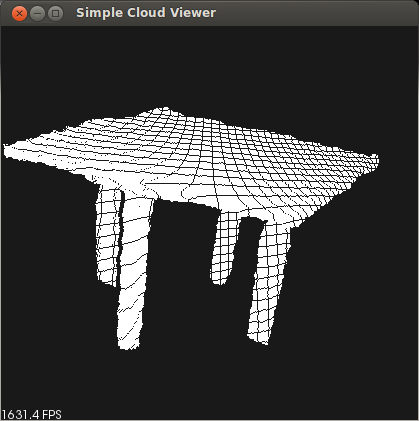
\includegraphics[width=0.30\textwidth]{figures/mesa2_1.png}
	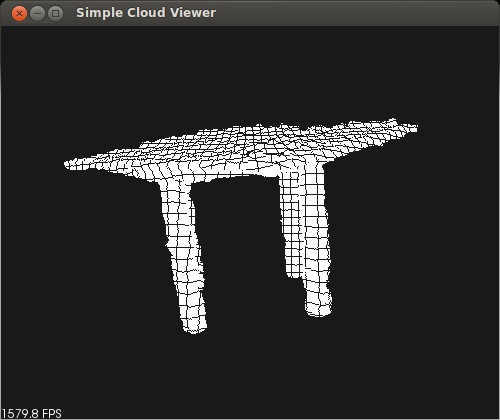
\includegraphics[width=0.30\textwidth]{figures/mesa2_2.png}
	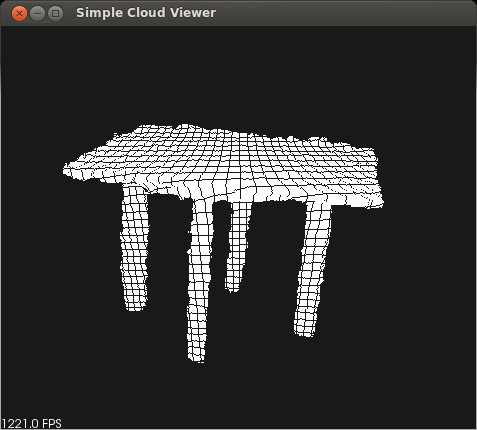
\includegraphics[width=0.30\textwidth]{figures/mesa2_3.png}
	\captionof{figure}{Clusters representativos da mesa 2.}
	\label{fig:mesa2_ensaios}
\end{center}
\end{figure}


\begin{table}[htb]
\begin{center}
\begin{tabular} { c c c c c | c }
	Modelo do dicionário & \(C_1\) & \(C_2\) & \(C_n\) & \(C_h\) & \(C\) \\
	\hline
	\multicolumn{6}{ c }{Primeiro Ensaio}\\
	\hline
	Mesa 1 &	 0.423086 &	0.664045 & 1.000000 & 0.375991 & 0.584580 \\
	Mesa 2 &	 0.596547 &	0.811000 & 1.000000 & 0.365248 & 0.661461 \\
	Mesa 3 &	 0.596547 &	0.811000 & 1.000000 & 0.433345 & 0.681890 \\
	Mesa 4 &	 0.701727 &	0.792667 & 0.666667 & 0.284082 & 0.592156 \\
	Mesa 5 &	 0.935636 &	0.792667 & -2.000000 & 0.319592 & 0.127953 \\
	\hline
	\multicolumn{6}{ c }{Segundo Ensaio}\\
	\hline
	Mesa 1 &	 0.490549 &	0.612359 & 0.750000 & 0.440277 & 0.557810 \\
	Mesa 2 &	 0.656589 &	0.765000 & 0.750000 & 0.427698 & 0.633707 \\
	Mesa 3 &	 0.656589 &	0.765000 & 0.750000 & 0.507438 & 0.657629 \\
	Mesa 4 &	 0.671706 &	0.823333 & 1.000000 & 0.332654 & 0.673556 \\
	Mesa 5 &	 0.895608 &	0.823333 & -1.000000 & 0.374236 & 0.342006 \\
	\hline
	\multicolumn{6}{ c }{Terceiro Ensaio}\\
	\hline
	Mesa 1 &	 0.610414 &	0.776405 & 1.000000 & 0.288464 & 0.633244 \\
	Mesa 2 &	 0.763269 &	0.911000 & 1.000000 & 0.280222 & 0.702634 \\
	Mesa 3 &	 0.763269 &	0.911000 & 1.000000 & 0.332467 & 0.718307 \\
	Mesa 4 &	 0.618366 &	0.726000 & 0.666667 & 0.217950 & 0.534810 \\
	Mesa 5 &	 0.824488 &	0.726000 & -2.000000 & 0.245194 & 0.061180 \\
	\hline
\end{tabular}
	\caption{Resultados da análise da Mesa 3}
	\label{res:mesa3}
\end{center}
\end{table}

O resultado desta análise \ref{res:mesa3} é também bastante satisfatório pois permite a identificação correta da mesa em análise na maioria dos casos: mesa 3.



\begin{figure}[htb]
\begin{center}
	\includegraphics[width=0.30\textwidth]{figures/mesa3_1.png}
	\includegraphics[width=0.30\textwidth]{figures/mesa3_2.png}
	\includegraphics[width=0.30\textwidth]{figures/mesa3_3.png}
	\captionof{figure}{Clusters representativos da mesa 3.}
	\label{fig:mesa3_ensaios}
\end{center}
\end{figure}



Os resultados são satisfatórios, pois pelos dados extraídos pode-se concluir que com uma técnica de identificação bastante simples, apesar de extensível, é possível reconhecer com sucesso uma mesa, cuja morfologia tenha sido previamente guardada.
Um dos grandes defeitos é o tempo que o pré-processamento demora, que a ser melhorado permitiria o rápido reconhecimento das mesas criando uma vantagem significativa no reconhecimento de objetos complexos.


\subsection{Tempos de Processamento}

Os tempos de processamento são de extrema importância pois avaliam a adequação da solução ao âmbito da robótica autónoma, pois este requer baixos tempos de execução para fazer rapidamente a identificação de objetos.

\begin{table}[htb]
\begin{center}
\begin{tabular} { l | c c }
	\multicolumn{3}{ c }{ Tempos de processamento}\\
	Ensaio & Pré processamento (s) & Identificação (s)\\
	\hline
	1 & 11.840000 & 0.41 \\
	2 &  8.530000 & 0.40 \\
	3 & 18.770000 & 0.46 \\
	\hline
\end{tabular}
	\caption{Tempos de processamento da análise da Mesa 1}
	\label{res:mesa1_tempo}
\end{center}
\end{table}

Como se vê na tabela~\ref{res:mesa1_tempo} a maior parte do tempo de execução é passado no pré processamento, sendo a comparação com os modelos do dicionário feita de uma forma praticamente instantânea.

\begin{table}[htb]
\begin{center}
\begin{tabular} { l | c c }
	\multicolumn{3}{ c }{ Tempos de processamento}\\
	Ensaio & Pré processamento (s) & Identificação (s)\\
	\hline
	1 & 39.330000 & 1.02 \\
	2 & 13.460000 & 0.83 \\
	3 & 24.620000 & 0.74 \\
	\hline
\end{tabular}
	\caption{Tempos de processamento da análise da Mesa 2}
	\label{res:mesa2_tempo}
\end{center}
\end{table}

Verifica-se a tendência do pré-processamento ser bastante custoso, oscilando aqui entre aproximadamente 40 segundos e 13 segundos, enquanto que a identificação demora sempre aproximadamente 1 segundo.

\begin{table}[htb]
\begin{center}
\begin{tabular} { l | c c }
	\multicolumn{3}{ c }{ Tempos de processamento}\\
	Ensaio & Pré processamento (s) & Identificação (s)\\
	\hline
	1 & 35.510000 & 0.24 \\
	2 & 39.630000 & 0.24 \\
	3 & 62.590000 & 0.36 \\
	\hline
\end{tabular}
	\caption{Tempos de processamento da análise da Mesa 3}
	\label{res:mesa3_tempo}
\end{center}
\end{table}

Nos tempos de processamento para uma imagem RGBD com a Mesa 3 confirma-se que o tempo de pré processamento é bastante significativo, e apesar de absolutamente necessário acaba por atrasar o mais importante da questão que é a identificação do objeto.



%\section{Resumo}

\chapter{Conclusões e Trabalho Futuro} \label{chap:concl}

\section*{}

Deve ser apresentado um resumo do trabalho realizado e apreciada a
satisfação dos objetivos do trabalho, uma lista de contribuições
principais do trabalho e as direções para trabalho futuro.

A escrita deste capítulo deve ser orientada para a total compreensão
do trabalho, tendo em atenção que, depois de ler o Resumo e a
Introdução, a maioria dos leitores passará à leitura deste capítulo de
conclusões e recomendações para trabalho futuro.

\section{Satisfação dos Objectivos}

 

\section{Trabalho Futuro}

No que diz respeito a trabalho futuro, existem várias melhorias que poderiam ser introduzidas, contudo as mais concretas seriam em dois campos muito particulares: rapidez de reconhecimento e a forma como a avaliação é realizada.

No que diz respeito à rapidez de reconhecimento, tendo em conta que a rapidez de identificação é um requisito muito importante no que diz respeito à robótica autónoma, poder-se-á potenciar a velocidade de reconhecimento usando bibliotecas de paralelização (como a OpenMP) para avaliar os \emph{clusters}, encontrados na imagem, em paralelo. Outra das hipóteses seria usar, por exemplo, algoritmos genéticos para otimizar os fatores envolvidos na deteção de \emph{clusters} pois é a operação mais custosa em termos de tempo no processo global\footnote{fundamentar com dados}.

Quanto à avaliação, 



%\vspace*{12mm}


 

%%----------------------------------------
%% Final materials
%%----------------------------------------

\begin{singlespace}
  %% Bibliography
  %% Comment the next command if BibTeX file not used; bibliography is in ``myrefs.bib''
  \PrintBib{myrefs}

  %% Index
  %% Uncomment next command if index is required, don't forget to run ``makeindex mieic'' command
  \PrintIndex

  %% Comment next 2 commands if numbered appendixes not used
  %\appendix
  %\chapter{Loren Ipsum} \label{ap1:loren}

Depois das conclusões e antes das referências bibliográficas,
apresenta-se neste anexo numerado o texto usado para preencher a
dissertação.

\section{O que é o \emph{Loren Ipsum}?}

\emph{\textbf{Lorem Ipsum}} is simply dummy text of the printing and
typesetting industry. Lorem Ipsum has been the industry's standard
dummy text ever since the 1500s, when an unknown printer took a galley
of type and scrambled it to make a type specimen book. It has survived
not only five centuries, but also the leap into electronic
typesetting, remaining essentially unchanged. It was popularised in
the 1960s with the release of Letraset sheets containing Lorem Ipsum
passages, and more recently with desktop publishing software like
Aldus PageMaker including versions of Lorem Ipsum~\citep{kn:Lip08}. 

\section{De onde Vem o Loren?}

Contrary to popular belief, Lorem Ipsum is not simply random text. It
has roots in a piece of classical Latin literature from 45 BC, making
it over 2000 years old. Richard McClintock, a Latin professor at
Hampden-Sydney College in Virginia, looked up one of the more obscure
Latin words, consectetur, from a Lorem Ipsum passage, and going
through the cites of the word in classical literature, discovered the
undoubtable source. Lorem Ipsum comes from sections 1.10.32 and
1.10.33 of ``de Finibus Bonorum et Malorum'' (The Extremes of Good and
Evil) by Cicero, written in 45 BC. This book is a treatise on the
theory of ethics, very popular during the Renaissance. The first line
of Lorem Ipsum, ``Lorem ipsum dolor sit amet\ldots'', comes from a line in
section 1.10.32.

The standard chunk of Lorem Ipsum used since the 1500s is reproduced
below for those interested. Sections 1.10.32 and 1.10.33 from ``de
Finibus Bonorum et Malorum'' by Cicero are also reproduced in their
exact original form, accompanied by English versions from the 1914
translation by H. Rackham.

\section{Porque se usa o Loren?}

It is a long established fact that a reader will be distracted by the
readable content of a page when looking at its layout. The point of
using Lorem Ipsum is that it has a more-or-less normal distribution of
letters, as opposed to using ``Content here, content here'', making it
look like readable English. Many desktop publishing packages and web
page editors now use Lorem Ipsum as their default model text, and a
search for ``lorem ipsum'' will uncover many web sites still in their
infancy. Various versions have evolved over the years, sometimes by
accident, sometimes on purpose (injected humour and the like). 

\section{Onde se Podem Encontrar Exemplos?}

There are many variations of passages of Lorem Ipsum available, but
the majority have suffered alteration in some form, by injected
humour, or randomised words which don't look even slightly
believable. If you are going to use a passage of Lorem Ipsum, you need
to be sure there isn't anything embarrassing hidden in the middle of
text. All the Lorem Ipsum generators on the Internet tend to repeat
predefined chunks as necessary, making this the first true generator
on the Internet. It uses a dictionary of over 200 Latin words,
combined with a handful of model sentence structures, to generate
Lorem Ipsum which looks reasonable. The generated Lorem Ipsum is
therefore always free from repetition, injected humour, or
non-characteristic words etc. 

\end{singlespace}

\end{document}
